

The success of a mixed finite element formulation crucially depends on a proper choice of the local interpolations of the velocity and the pressure. 

%........................................................................................
\subsubsection{The compatibility condition (or LBB condition, or inf-sup condition)} \label{ss:LBBcond}
\index{general}{LBB} \index{general}{Optimal Rate}

\begin{flushright} {\tiny {\color{gray} lbb.tex}} \end{flushright}
%~~~~~~~~~~~~~~~~~~~~~~~~~~~~~~~~~~~~~~~~~~~~~~~~~~~~~~~~~~~~~~~~~~~~~~~~~~~~~~~~~~~~~~~~~~~~~~~~~~

WARNING: I am not comfortable (yet) writing about this topic. 
What follows is a rough attempt at making sense of it.

\hspace{.4cm}

The Lady{\v z}henskaya-Babu{\v s}ka-Brezzi (LBB\footnote{
\url{https://en.wikipedia.org/wiki/Ladyzhenskaya-Babuska-Brezzi_condition}}) condition is a sufficient 
condition for a saddle point problem to have a unique solution.
For saddle point problems coming from the Stokes equations, 
many discretizations (i.e. choices for the velocity and pressure polynomial spaces)
are unstable, giving rise to artifacts such as spurious oscillations. 
The LBB condition gives criteria for when a discretization of a saddle point problem is stable. 
It also assures convergence at the optimal rate. 

Bochev \& Gunzburger \cite{bogu09} state: ``
The terminology 'LBB' originates from the facts that this condition was first explicitly discussed
in the finite element setting for saddle point problems by Brezzi\footnote{
\url{https://en.wikipedia.org/wiki/Franco_Brezzi}} \cite{brez74} and that it is a special case of
the general weak-coercivity condition first discussed for finite element methods by Ivo Babu{\v s}ka\footnote{
\url{https://en.wikipedia.org/wiki/Ivo_Babuska}}
\cite{babu71} and that, in the continuous setting of the Stokes equation, this condition was first proved to
hold by Olga Ladyzhenskaya\footnote{\url{https://en.wikipedia.org/wiki/Olga_Ladyzhenskaya}}; see \cite{lady69}.''

Unfortunately, to quote Donea \& Huerta \cite{dohu03}: 
``In the finite element context, it is by no means easy to prove whether or not a given
velocity-pressure pair satisfies the LBB compatibility condition.''
Elman \etal state: ``[...] Choosing spaces for which the discrete inf-sup condition holds
and is a delicate matter, and seemingly natural choices of velocity and pressure approximation
do not work. [...] In general, care must be taken to make the velocity space 
rich enough compared to the pressure space.'' By rich enough the authors essentially mean that 
the order of the polynomials used to represent velocity must be higher than the one used 
for pressure.

The LBB condition, or inf-sup condition can be proven in different ways, 
and standard techniques have been designed
as listed in Boffi \etal (2008) \cite{bobf08}.

%p129
Elman \etal \cite{elsw} state that ``The inf-sup condition is a sufficient condition 
for the pressure to be unique up to constant in the case of an enclosed flow.''
This can also be proven for other boundary conditions.
This approach, based on the macro-element technique \cite{sten90} is explored in Appendix \ref{app:Gel}.

It can be shown that, provided the kernel (null space) of matrix $\G$ is zero,
the Stokes matrix is non-singular, that is $\vec{\cal V}$ and $\vec{\cal P}$ 
are uniquely defined, and the Schur complement matrix $\SSS$ is positive definite. 
Simply put, taking $\vec{\cal V}=\vec{0}$ in the discretised Stokes system 
without body forces yields $\G \cdot \vec{\cal P}=\vec{0}$ and implies
that any pressure solution is only unique up to the null space of the matrix $\G$.

We know that the Schur complement matrix $\SSS$ is positive definite if and only if all of its eigenvalues are positive.
One could then (numerically) compute the eigenvalues of $\SSS$ and check that these are indeed strictly positive
to show that $\SSS$ is positive definite but that would prove very costly. 

Another way is to see that $\SSS$ is positive definite only if $\text{ker}(\G)=\{0\}$.
Again to quote Donea \& Huerta \cite{dohu03}: ``If this is the case, the partitioned Stokes matrix  
is non-singular and delivers uniquely defined velocity and pressure fields. If this is not the case, a
stable and convergent velocity field might be obtained, but the pressure field is likely
to present spurious and oscillatory results.'' 
Note that in the case of the ${\bm Q}_1 \times P_0$ element it has been shown that the multiple families of 
checkboard pressure modes actually lie in the kernel of $\G$. \cite{sagl81a,sagl81b}

\hspace{.4cm}

We can look at this in a different manner, as explained in \textcite{elsw}:
the unique solvability of the matrix system
\begin{equation}
\left(
\begin{array}{cc}
\K & \G \\
\G^T & 0 
\end{array}
\right)
\cdot 
\left(
\begin{array}{c}
\vec{\cal V} \\ \vec{\cal P}
\end{array}
\right)
=
\left(
\begin{array}{c}
\vec{f} \\ \vec{h}
\end{array}
\right)
\label{eq:lbbsyst}
\end{equation}
is determined by looking at the homogeneous system
\begin{equation}
\left(
\begin{array}{cc}
\K & \G \\
\G^T & 0 
\end{array}
\right)
\cdot 
\left(
\begin{array}{c}
\vec{\cal V} \\ \vec{\cal P}
\end{array}
\right)
=
\left(
\begin{array}{c}
\vec{0} \\ \vec{0}
\end{array}
\right)
\end{equation}
or,
\begin{eqnarray}
\K \cdot \vec{\cal V} + \G \cdot \vec{\cal P} &=& \vec{0} \nn\\
\G^T \cdot \vec{\cal V} &=& \vec{0}
\end{eqnarray}
To start, premultiply the first equation by $\vec{\cal V}^T$ and the second by 
$\vec{\cal P}^T$. The second yields
$\vec{\cal P}^T \cdot \G^T \cdot \vec{\cal V} = ( \vec{\cal V}^T \cdot \G\cdot \vec{\cal P}  )^T = \vec{0}$
which is present in the first equation so that it simplifies to $\vec{\cal V}^T\cdot \K \cdot \vec{\cal V} = \vec{0}$.
Since $\K$ is positive definite, it follows that $\vec{\cal V}=\vec{0}$, implying unique solvability
with respect to the velocity. 

On the other hand, unique solvability with respect to the pressure is problematic. Substituting $\vec{\cal V}=\vec{0}$
in the system above gives $\G \cdot \vec{\cal P} = \vec{0}$, and implies that any pressure solution is only unique 
up to the nullspace of the matrix $\G$. 
The bottom line is that if Eq.~\eqref{eq:lbbsyst} is to properly represent a continuous Stokes
problem, then the mixed approximation spaces need to be chosen carefully.
Specifically, we have to ensure that $\text{null}(\G)=\{1\}$ in the case of enclosed flow,
and that $\text{null}(\G)=\{0\}$, otherwise.

\textcite{grsa} state: ``LBB stable elements assure the existence of a unique solution to Stokes flow and 
assure convergence at optimal rate. [...] LBB-unstable elements may not converge, and if they do, they may not do so at the optimal rate.''



%........................................................................................
\subsubsection{Families}
\index{general}{Taylor-Hood}

The family of {\color{olive} Taylor-Hood} finite element spaces on triangular/tetrahedral 
grids is given by ${\bm P}_k \times P_{k-1}$ with $k\geq 2$, 
and on quadrilateral/hexahedral grids by ${\bm Q}_k \times Q_{k-1}$ with $k\geq 2$.
This means that the pressure is then approximated by continuous functions. 

These finite elements are very popular, in particular the pairs for $k=2$, i.e.
${\bm Q}_2\times Q_1$ and ${\bm P}_2\times P_1$.
The reason why $k\geq 2$ comes from the fact that the 
${\bm Q}_1 \times Q_0$ (often referred to as ${\bm Q}_1 \times P_0$) and ${\bm P}_1\times P_0$
are not stable elements (they are not inf-sup stable), as
shown in John \cite[p64]{john16} and \cite[p67]{john16}. 

\begin{remark}
Note that a similar element to ${\bm Q}_2 \times Q_1$ has been proposed
and used succesfully used in \textcite{taho73} (1973) and \textcite{hota74} (1974): 
it is denoted by ${\bm Q}_2^{(8)} \times Q_1$ 
since the center node ('$x^2y^2$') and its associated degrees of freedom have been removed. It 
has also been proved to be LBB stable. These are also called {\color{olive} Serendipity} elements. 
\end{remark}

%........................................................................................
\subsubsection{The bi/tri-linear velocity - constant pressure element ($Q_1\times P_0$)}
\label{ss:pairq1p0}
\begin{flushright} {\tiny {\color{gray} pair\_q1p0.tex}} \end{flushright}
%~~~~~~~~~~~~~~~~~~~~~~~~~~~~~~~~~~~~~~~~~~~~~~~~~~~~~~~~~~~~~~~~~~~~~~~~~~~~~~~~~~~~~~~~~~~~~~~~~~


\begin{minipage}{0.48\textwidth}
\begin{center}
\begin{flushright} {\tiny {\color{gray} (tikz\_q1p0.tex)}} \end{flushright}
%~~~~~~~~~~~~~~~~~~~~~~~~~~~~~~~~~~~~~~~~~~~~~~~~~~~~~~~~~~~~~~~~~~~~~~~~~~~~~~~~~~~~~~~~~~~~~~~~~~

\begin{tikzpicture}
%\draw[fill=gray!23,gray!23](0,0) rectangle (5,5);
%\draw[step=0.5cm,gray,very thin] (0,0) grid (4,4); %background grid
\draw[thick] (1,1) -- (3,1.2) -- (2.7,3) -- (1.1,3.1) -- cycle;  
\node[] at (0.8,0.8) {0};
\node[] at (3.2,1) {1};
\node[] at (2.9,3.1) {2};
\node[] at (0.9,3.2) {3};
\draw[violet] (1.9,2.075) circle (4pt);
\draw[black,fill=teal] (1,1)   circle (2pt);
\draw[black,fill=teal] (3,1.2)  circle (2pt);
\draw[black,fill=teal] (2.7,3)  circle (2pt);
\draw[black,fill=teal] (1.1,3.1) circle (2pt);
\draw[black,fill=teal] (3.1,0.2) circle (2pt); 
\node[] at (3.4,0.2) {$\vec\upnu$};
\draw[violet] (4.1,0.2) circle (4pt); 
\node[] at (4.4,0.2) {$p$};
\node[] at (2.5,4.5) {4 vel. nodes, 1 press. node};
\end{tikzpicture}

\end{center}
\end{minipage}
\begin{minipage}{0.48\textwidth}
\begin{center}

\begin{tikzpicture}
%\draw[fill=gray!23,gray!23](0,0) rectangle (5,5);
%\draw[step=0.25cm,gray,very thin] (0,0) grid (5,4); %background grid
\draw[thick] (1,0.5) -- (3.25,0.75) -- (3,3) -- (0.5,2.5) -- cycle; %1-2-6-5
\draw[thick] (3.25,0.75) -- (4,1.5) -- (4.25,3.75) -- (3,3) -- cycle; %2-3-7-6
\draw[thick] (0.5,2.5) -- (3,3) -- (4.25,3.75) -- (1.75,3.5) -- cycle; %5-6-7-4
\draw[thin]   (1,0.5) -- (2,1.75) -- (1.75,3.5) -- (0.5,2.5)   --cycle; % 1-0-4-5 
\draw[thin] (2,1.75) -- (4,1.5); 
%\node[] at (0.8,0.8) {0};
%\node[] at (3.2,1) {1};
%\node[] at (2.9,3.1) {2};
%\node[] at (0.9,3.2) {3};
\draw[violet] (2.5,2.) circle (4pt);
\draw[black,fill=teal] (1,0.5)   circle (2pt);
\draw[black,fill=teal] (3.25,0.75)   circle (2pt);
\draw[black,fill=teal] (3,3)   circle (2pt);
\draw[black,fill=teal] (0.5,2.5)   circle (2pt);
\draw[black,fill=teal] (1.75,3.5)  circle (2pt);
\draw[black,fill=teal] (4.25,3.75)  circle (2pt);
\draw[black,fill=teal] (4,1.5) circle (2pt);
\draw[black,fill=teal] (2,1.75) circle (2pt);
\draw[black,fill=teal] (3.1,0.2) circle (2pt); 
\node[] at (3.4,0.2) {$\vec\upnu$};
\draw[violet] (4.1,0.2) circle (4pt); 
\node[] at (4.4,0.2) {$p$};
\node[] at (2.5,4.5) {8 vel. nodes, 1 press. node};
\end{tikzpicture}

\end{center}
\end{minipage}

However simple it may look, the \index{general}{${\bm Q}_1 \times P_0$} element is 
one of the hardest elements to analyze and many questions are still open about its properties. 
The element does not satisfy the inf-sup condition \cite[p211]{hugh}. 
In Gresho \& Sani \cite{grsa} it is labeled as follows: ``slightly unstable but highly usable''. 

The ${\bm Q}_1 \times P_0$ mixed approximation is the lowest order conforming approximation 
method defined on a rectangular grid. It also happens to be the most famous example 
of an unstable mixed approximation method \cite[p235]{elsw}.
\textcite{boni84} (1984) and \textcite{boni85} (1985) show that it is not stable.

This element is discussed in Fortin (1981) \cite{fort81}, Fortin \& Fortin (1985) \cite{fofo85} 
and in Pitk\"aranta \& Saarinen (1985) \cite{pisa85} in the context of multigrid use.

This element is plagued by so-called pressure checkerboard modes which
have been thoroughly analysed, see for example \textcite{grsi94} (1994), 
\textcite{chpc95} (1995), \textcite{sagl81a,sagl81b} (1981).
These can be filtered out, see for example \textcite{chpc95} (1995) or \textcite{legs79} (1997), 
and explained in Section~\ref{psmoothing}.

\Literature: \textcite{fobo90} (1990), \cite{grle85} (1985),
\textcite{leru86} (1986), \textcite{odja84} (1984).



%----------------------------------------------------------------------
\subsubsection{The bi/tri-quadratic velocity - bi/tri-linear pressure element ($Q_2 \times Q_1$)}
\label{ss:pairq2q1}
\begin{flushright} {\tiny {\color{gray} pair\_q2q1.tex}} \end{flushright}
%~~~~~~~~~~~~~~~~~~~~~~~~~~~~~~~~~~~~~~~~~~~~~~~~~~~~~~~~~~~~~~~~~~~~~~~~~~~~~~~~~~~~~~~~~~~~~~~~~~

\noindent
\begin{minipage}{0.48\textwidth}
\begin{center}
\begin{flushright} {\tiny {\color{gray} (tikz\_q2q1.tex)}} \end{flushright}
%~~~~~~~~~~~~~~~~~~~~~~~~~~~~~~~~~~~~~~~~~~~~~~~~~~~~~~~~~~~~~~~~~~~~~~~~~~~~~~~~~~~~~~~~~~~~~~~~~~

%\begin{center}
\begin{tikzpicture}
%\draw[fill=gray!23,gray!23](0,0) rectangle (5,5);
%\draw[step=0.5cm,gray,very thin] (0,0) grid (4,4); %background grid
\draw[thick] (1,1) -- (3,1.2) -- (2.7,3) -- (1.1,3.1) -- cycle;  
\node[] at (0.7,0.8) {0};
\node[] at (3.3,1) {1};
\node[] at (3,3.1) {2};
\node[] at (0.8,3.2) {3};
\draw[black,fill=teal] (1,1)     circle (2pt); \draw[violet] (1,1) circle (4pt);
\draw[black,fill=teal] (3,1.2)   circle (2pt); \draw[violet] (3,1.2) circle (4pt);
\draw[black,fill=teal] (2.7,3)   circle (2pt); \draw[violet] (2.7,3) circle (4pt);
\draw[black,fill=teal] (1.1,3.1) circle (2pt); \draw[violet] (1.1,3.1) circle (4pt);
\draw[black,fill=teal] (2,1.1) circle (2pt) ; \node[] at (2,0.8) {4};
\draw[black,fill=teal] (2.85,2.1) circle (2pt) ; \node[] at (3.1,2.1) {5};
\draw[black,fill=teal] (1.9,3.05) circle (2pt) ; \node[] at (1.9,3.3) {6};
\draw[black,fill=teal] (1.05,2.05) circle (2pt) ; \node[] at (0.8,2) {7};
\draw[black,fill=teal] (1.9,2.075) circle (2pt) ; \node[] at (2.1,2) {8};
\draw[black,fill=teal] (3.1,0.2) circle (2pt); 
\node[] at (3.4,0.2) {$\vec\upnu$};
\draw[violet] (4.1,0.2) circle (4pt); 
\node[] at (4.4,0.2) {$p$};
\node[] at (2.5,4.5) {9 vel. nodes, 4 press. nodes};
\end{tikzpicture}
%\end{center}

\end{center}
\end{minipage}
\hfill
\begin{minipage}{0.48\textwidth}
\begin{center}



%\begin{center}
\begin{tikzpicture}
%\draw[fill=gray!23,gray!23](0,0) rectangle (5,5);
%\draw[step=0.5cm,gray,very thin] (0,0) grid (5,4); %background grid
\draw[thick] (1,0.5) -- (2,0.55) --(3.25,0.75) -- (3,3) -- (0.5,2.5) -- cycle; %1-9-2-6-5
\draw[thick] (3.25,0.75) -- (3.6,1.05) -- (4,1.5) -- (4.25,3.75) -- (3,3) -- cycle; %2-10-3-7-6
\draw[thick] (0.5,2.5) -- (3,3) -- (4.25,3.75) -- (1.75,3.5) -- (1.1,3.1) -- cycle; %5-6-7-4-13
\draw[thin]   (1,0.5) -- (1.5,1.25) -- (2,1.75) -- (1.75,3.5) -- (1.1,3.1) -- (0.5,2.5) --cycle; % 1-8-0-4-5-13 
\draw[thin] (2,1.75) -- (3,1.75) -- (4,1.5); %0-11-3
%pressure nodes
\draw[violet] (2,1.75) circle (4pt); % 0 
\draw[violet] (1,0.5) circle (4pt); % 1 
\draw[violet] (3.25,0.75) circle (4pt); % 2 
\draw[violet] (4,1.5) circle (4pt); % 3 
\draw[violet] (1.75,3.5) circle (4pt); % 4 
\draw[violet] (0.5,2.5) circle (4pt); % 5 
\draw[violet] (3,3) circle (4pt); % 6 
\draw[violet] (4.25,3.75) circle (4pt); % 7 
%velocity nodes
\draw[black,fill=teal] (1,0.5)   circle (2pt);
\draw[black,fill=teal] (3.25,0.75)   circle (2pt);
\draw[black,fill=teal] (3,3)   circle (2pt);
\draw[black,fill=teal] (0.5,2.5)   circle (2pt);
\draw[black,fill=teal] (1.75,3.5)  circle (2pt);
\draw[black,fill=teal] (4.25,3.75)  circle (2pt);
\draw[black,fill=teal] (4,1.5) circle (2pt);
\draw[black,fill=teal] (2,1.75) circle (2pt);
\draw[black,fill=teal] (1.5,1.25) circle (2pt); % 8 
\draw[black,fill=teal] (2,0.55) circle (2pt); % 9 
\draw[black,fill=teal] (3.6,1.05) circle (2pt); % 10
\draw[black,fill=teal] (3,1.75) circle (2pt); % 11
\draw[black,fill=teal] (0.75,1.5) circle (2pt); % 12
\draw[black,fill=teal] (1.1,3.1) circle (2pt); % 13
\draw[black,fill=teal] (0.75,1.5) circle (2pt); % 18
\draw[black,fill=teal] (2.7,1.1) circle (2pt); % 21
\draw[black,fill=teal] (3.6,3.35) circle (2pt); % 21
\draw[black,fill=teal] (3.,3.62) circle (2pt); % 21
\draw[black,fill=teal] (4.12,2.6) circle (2pt); % 21
\draw[black,fill=teal] (1.89,2.5) circle (2pt); % 21
\draw[black,fill=teal] (1.75,2.75) circle (2pt); % 21
\draw[black,fill=teal] (3.12,1.9) circle (2pt); % 21
\draw[black,fill=teal] (3.6,2.2) circle (2pt); % 21
\draw[black,fill=teal] (1.25,2.1) circle (2pt); % 21
\draw[black,fill=teal] (2.4,3.2) circle (2pt); % 21
\draw[black,fill=teal] (2.5,2.5) circle (2pt); % 21

% legend
\draw[black,fill=teal] (3.1,0.2) circle (2pt); \node[] at (3.4,0.2) {$\vec\upnu$};
\draw[violet] (4.1,0.2) circle (4pt); 
\node[] at (4.4,0.2) {$p$};
\node[] at (2.5,4.5) {27 vel. nodes, 8 press. nodes};
\end{tikzpicture}
%\end{center}


\end{center}
\end{minipage}

It belongs to the Taylor-Hood family of elements and satisfies the inf-sup (LBB) condition \cite[p215]{hugh}.
Gresho \& Sani \cite[p554]{grsa} write that in their opinion $div(\vec v)=0$ is not strong enough.
This element, implemented in penalised form, is discussed in Bercovier \& Engelman (1979) \cite{been79} 
and the follow-up paper \cite{been80}. 

It is the default of the \aspect code (see Appendix~\ref{app:codes}).
It is implemented in \stone~18,21,48,91,120,...
 




%----------------------------------------------------------------------
\subsubsection{The bi/tri-quadratic velocity - discontinuous linear pressure element ($Q_2 \times P_{-1}$)}
\label{ss:pairq2pm1}

\noindent
\begin{minipage}{0.58\textwidth}


This element is crowned "probably the most accurate 2D element" 
in Gresho \& Sani \cite{grsa}.

It is characterised by piecewise Biquadratic velocities, 
and piecewise linear discontinuous polynomial pressure. 
The element satisfies the inf-sup condition, see page 211 of Hughes \cite{hugh}, or 
p138 of Elman \etal \cite{elsw}.
It is used in van de Vosse \etal (1989) \cite{vavs89} for steady laminar flow in a curved tube. 

See Boffi \& Gastaldi (2002) \cite{boga02} 
for the two possible choices for the two definitions of the pressure space (mapped and un-mapped), 
and check \stone~76 for their implementation.

This element is mentioned in Kaus (2010) \cite{kaus10} and Pelletier \etal (1989) \cite{pefc89} 
and it is  used in Frehner (2014) \cite{freh14} to study 3D fold growth rates 
(see online supplementary material) and in Schmalholtz (2008) \cite{schm08}.

Note that the serendipity version of this pair, i.e. $Q_2^{(20)}\times P_{-1}$ is also LBB stable
as shown in p180 of Reddy \cite{reddybook2}.

\end{minipage}
\hfill
\begin{minipage}{0.38\textwidth}
\begin{center}
\begin{flushright} {\tiny {\color{gray} (tikz\_p2pm1.tex)}} \end{flushright}
%~~~~~~~~~~~~~~~~~~~~~~~~~~~~~~~~~~~~~~~~~~~~~~~~~~~~~~~~~~~~~~~~~~~~~~~~~~~~~~~~~~~~~~~~~~~~~~~~~~


%\begin{center}
\begin{tikzpicture}
%\draw[fill=gray!23,gray!23](0,0) rectangle (5,5);
%\draw[step=0.5cm,gray,very thin] (0,0) grid (5,5); %background grid
\draw[thick] (1,1) -- (4,1) -- (4,3) -- (1,3) -- cycle;  
\node[] at (0.7,0.8) {0};
\node[] at (4.3,0.8) {1};
\node[] at (4.25,3.1) {2};
\node[] at (0.8,3.2) {3};
\draw[black,fill=teal] (1,1)     circle (2pt); 
\draw[black,fill=teal] (4,1)   circle (2pt); 
\draw[black,fill=teal] (4,3)   circle (2pt); 
\draw[black,fill=teal] (1,3) circle (2pt); 
\draw[black,fill=teal] (2.5,1) circle (2pt) ; 
\draw[black,fill=teal] (2.5,3) circle (2pt) ; 
\draw[black,fill=teal] (1,2) circle (2pt) ; 
\draw[black,fill=teal] (4,2) circle (2pt) ; 

\draw[violet] (2.5,2) circle (4pt);
\draw[violet] (3,2) circle (4pt);
\draw[violet] (2.5,2.5) circle (4pt);

\draw[black,fill=teal] (3.1,0.2) circle (2pt); 
\node[] at (3.4,0.2) {$\vec\upnu$};
\draw[violet] (4.1,0.2) circle (4pt); 
\node[] at (4.4,0.2) {$p$};
\node[] at (2.5,3.85) {9 vel. nodes, 3 press. nodes};
\end{tikzpicture}
%\end{center}

\end{center}
\end{minipage}




%----------------------------------------------------------------------
\subsubsection{The biquadratic velocity - discontinuous bilinear pressure element ($Q_2 \times Q_{-1}$)}
\label{ss:pair_q2qm1}
This element is shown in Table~3.13-2 of Gresho \& Sani's book \cite{grsa}, 
and discussed in Section~3.13.6b of the book too. It is {\it not} LBB stable
and has one chequerboard pressure mode.

It is used (alongside many other element pairs) in \textcite{chgs02} (2002) in the context of 
a flow benchmark in a 2D box. The authors conclude that ``[...] the Q2-Q-1 element fared
slightly better than the Q2-P-1 . Most surprising, though, were the good results obtained with
the 'old' Taylor–Hood element, Q2-Q1 .''

It is also used in \textcite{grsu02} (2002) on a similar benchmark setup (8:1 thermal 
cavity problem) along with ${\bm Q}_1\times P_0$, ${\bm Q}_2\times P_{-1}$ and 
${\bm Q}_2\times Q_1$. The authors state that Q2Q-1 has div- stability problems
but ``produces excellent results and is still useful in general.''
They also state ``If the pesky-mode instability could be eciently dealt with, then the Q2xQ-1 element
should be employed over the Q2xP-1 -especially in 3D (we believe).''
Authors mention that it was also used in \textcite{dejo83} and that it ``performed
EXTREMELY WELL.''

 


%----------------------------------------------------------------------
\subsubsection{The stabilised bi/tri-linear velocity - constant pressure element ($Q_1\times P_0$-stab)}
\label{ss:pairq1p0stab}
\begin{flushright} {\tiny {\color{gray} pair\_q1p0stab.tex}} \end{flushright}
%~~~~~~~~~~~~~~~~~~~~~~~~~~~~~~~~~~~~~~~~~~~~~~~~~~~~~~~~~~~~~~~~~~~~~~~~~~~~~~~~~~~~~~~~~~~~~~~~~~

WARNING: this entire subsection is copied from an old document. It needs to be revised and 
updated. I intend to write a Stone implementing this element.

\Literature: Explore these 2 refs which I found after my q1p0-stab work of 2015 \cite{chke20,eguc03}

Many techniques have been proposed to stabilise this element:

\begin{itemize}
\item method ? : \cite{bbgs04},  \cite{bodg06} , \cite{bogl07}
\item stabilisation through macro-elements: \cite{fobo90}, \cite{leru86}, \cite{leta81}
\item local jump stabilisation: \cite{sike90}, \cite{kesi92,vibo92,qizh07,chri02,chco01,lisi12,lica06}
\item global jump stabilisation: \cite{hufr87}, \cite{nosi98}, \cite{dowa89} \cite{chco01}
\item supg like stabilisation: \cite{teos00}, \cite{tezd92,hufb86}
\item enrichment through velocity and/or pressure bubble function \cite{frol03}(only triangles)
\item additional (normal) velocity degrees of freedom on faces \cite{fofo85}, 
mentioned in \cite{sofo87}, \cite{fort81}.
adding 1 dof mid-side on each face with buble function \cite{rota87}
\end{itemize}

In effect, both jump stabilisation techniques provide an a-priori filter for the weakly unstable pressure modes associated 
with the Q1P0 element. The global jump stabilisation formulation introduces a pressure diffusion operator
that perturbs the incompressibility constraint. The global jump formulation insures mass conservation in a global  
sense since the null space of the stabilising matrix constains the constant-pressure vector. However, the global 
jump stabilisation smears the div-free constraint over a small region, i.e., the divergence is not 
zero at the element level \cite{chri00}.

The stability of mixed finite element methods boils down to properties of the null space of the matrix $\G$. 
An approximation is unstable if $\G \cdot \vec{\cal P} = \vec{0}$ where $\vec{\cal P}$ 
corresponds to some spurious pressure mode different from the constant value pressure.  
Note that if $\G\cdot \vec{\cal P} = \vec{0}$, then $(\vec{0},\vec{\cal P})^T$ is a null vector of 
the homogeneous system. 
The basic idea behind stabilization is to relax the incompressibility constraint in a special way so that 
this vector is no longer a null vector of the resulting coefficient matrix, and 
the discrete solutions satisfy rigorous error bounds. 
Stabilization is applicable to any mixed approximation method. 

Spatial discretisation of the Stokes equation using FD of FE results 
in large, sparse saddle-point systems of the form

\begin{equation}
\left(
\begin{array}{cc}
\K & \G \\
\G^T & -\C
\end{array}
\right)
\cdot
\left(
\begin{array}{c}
\vec{\cal V} \\ \vec{\cal P}
\end{array}
\right)
=
\left(
\begin{array}{c}
\vec{f} \\  \vec{h}
\end{array}
\right)
\end{equation}
where $\C$ is a stabilisation matrix to be stpecified.

The dimension of the $\C$ matrix is that of $h^{dim}/\eta$ where 
$h$ is the element size and $\eta$ a viscosity.







%----------------------------------------
\paragraph{Penalty approach}

The conventional way of computing a regularisation matrix $\C$
is to use a penalty formulation.
In the framework presented in \cite{sike90}, the standard penalty
method corresponds to the specific choice of
\[
C(q^h,p^h)=\epsilon \int_\Omega q^h p^h d\Omega = \epsilon {\bm M}_p
\]
with $\epsilon > 0$ and ${\bm M}_p$ is the pressure mass matrix. 
For a regular grid of squares with size $h$, it follows that 
\[
C_{ij}=0 \quad {\rm if} \; i\neq j
\quad\quad\quad
C_{ii}=\epsilon \int_{elt. i} d\Omega = h^2 \epsilon
\]
so that the stabilisation matrix is diagonal (see red matrix hereunder).

It is stressed here that the penalty technique does not stabilise an  
unstable mixed method \cite{sike90}. A small penalty parameter 
means that the original problem is solved quite accurately.

See \cite{cuss86} for some more details about the penalty method.

%-----------------------------------------------------
\paragraph{Global jump stabilisation}

Consider the stabilisation term
\[
C(q^h,p^h) = \beta h \sum_{s=1}^{N_s} \int_{\partial \Omega_s}[[ q^h ]]  [[p^h ]] ds
\]
in which $h$ is the mesh parameter (defined locally), $[[.]]$ is the jump operator,
and $\beta>0$ is a stabilising parameter. 
The summation is over all interior inter-element edges.

%from \cite{sike90}
To illustrate, consider element $9$ is the patch of equally  sized
squares represented here

\begin{center}
\begin{flushright} {\tiny {\color{gray} (tikz\_globaljump.tex)}} \end{flushright}
%~~~~~~~~~~~~~~~~~~~~~~~~~~~~~~~~~~~~~~~~~~~~~~~~~~~~~~~~~~~~~~~~~~~~~~~~~~~~~~~~~~~~~~~~~~~~~~~~~~

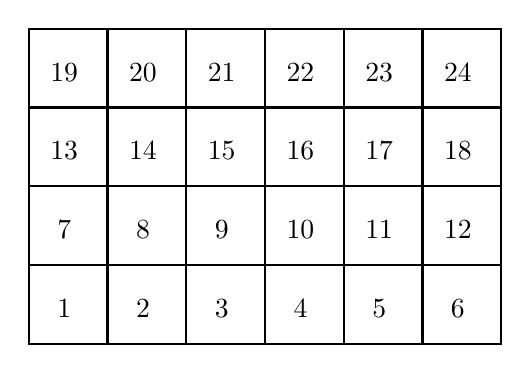
\begin{tikzpicture}
%\draw[step=0.5cm,gray,very thin] (0,0) grid (6,4); %background grid

\draw[thick] (0,0)--(6,0)--(6,4)--(0,4)--cycle;  

\draw[thick] (0,1)--(6,1);  
\draw[thick] (0,2)--(6,2);  
\draw[thick] (0,3)--(6,3);  

\draw[thick] (1,0)--(1,4);  
\draw[thick] (2,0)--(2,4);  
\draw[thick] (3,0)--(3,4);  
\draw[thick] (4,0)--(4,4);  
\draw[thick] (5,0)--(5,4);  

\node[] at (0.45,0.45) {1};
\node[] at (1.45,0.45) {2};
\node[] at (2.45,0.45) {3};
\node[] at (3.45,0.45) {4};
\node[] at (4.45,0.45) {5};
\node[] at (5.45,0.45) {6};

\node[] at (0.45,1.45) {7};
\node[] at (1.45,1.45) {8};
\node[] at (2.45,1.45) {9};
\node[] at (3.45,1.45) {10};
\node[] at (4.45,1.45) {11};
\node[] at (5.45,1.45) {12};

\node[] at (0.45,2.45) {13};
\node[] at (1.45,2.45) {14};
\node[] at (2.45,2.45) {15};
\node[] at (3.45,2.45) {16};
\node[] at (4.45,2.45) {17};
\node[] at (5.45,2.45) {18};

\node[] at (0.45,3.45) {19};
\node[] at (1.45,3.45) {20};
\node[] at (2.45,3.45) {21};
\node[] at (3.45,3.45) {22};
\node[] at (4.45,3.45) {23};
\node[] at (5.45,3.45) {24};

\end{tikzpicture}


\end{center}

The stabilisation term for this element involves the sum over its four neighbours:
\begin{eqnarray}
\beta h \sum_{s=1}^{4} \int_{\partial \Omega_s}[[ q^h ]]  [[p^h ]] ds
&=& \beta h^2 [ (p_9-p_3)+(p_9-p_8)+(p_9-p_{10})+(p_9-p_{15})   ]  \nn\\
&=& \beta h^2 ( 4 p_9-p_3 -p_8-p_{10} -p_{15})  \nn
\end{eqnarray}
The integral along each edge is simply the pressure difference across the edge 
multiplied by the edge surface/length which happens to be constant in this case.
This means that the in the matrix $\mathbb{C}$, there will be entries on the $9^{th}$
line at columns 3, 8, 10, and 15. 

Be careful, let us now turn to element 6: it has 2 neighbours (5 and 12), so that
the stabilisation term for this element involves the sum over its two neighbours:
\begin{eqnarray}
 \beta h^2 [ (p_6-p_5)+(p_6-p_{12})  ]  
&=& \beta h^2 ( 2 p_6-p_5 -p_{12} )  \nn
\end{eqnarray}

And looking now at element 23: it has three neighbours (17, 22, and 24), so that 
the stabilisation term for this element involves the sum over its three neighbours:
\begin{eqnarray}
\beta h^2 [ (p_{23}-p_{17})+(p_{23}-p_{22}) +(p_{23}-p_{24})  ] 
&=& \beta h^2 ( 3 p_{23}-p_{17} -p_{22} - p_{24} )  \nn
\end{eqnarray}


The resulting assembled $\C$ matrix is shown in green on the figure here after.

The global jump stabilisation is effective in
practice, although a careful choice of the parameter $\beta$
is required in order to prevent a loss of accuracy in the solution.
The only other deficiency is the fact that the global nature of the jump terms makes the method awkward to implement into existing codes
\footnote{I don't understand this remark}.\cite{sike90}

A general theoretical framework for analysing global stabilisation techniques is
presented in \cite{hufr87}.
Using this framework, optimum rates of convergence for the $Q_1\times P_0$
method stabilised with global jumps are established.

In \cite{cao03} the parameter $\beta$ is set to 1.

Note that this approach is somewhat linked to the idea of a pressure smoother 
via a discrete Laplace\footnote{\url{http://en.wikipedia.org/wiki/Discrete_Laplace_operator}}:
The Discrete Laplace operator is often used in image processing e.g. in edge detection and motion 
estimation applications. The discrete Laplacian is defined as the sum of the second derivatives Laplace 
and calculated as sum of differences over the nearest neighbours of the central pixel.
Here is an example of a 2D filter and it is of course similar in nature to the Global 
stabilisation stensil matrix:
\[
D^{(1)}=
\left[
\begin{array}{ccc}
0 &-1 &0\\
-1 &+4 &-1\\
0 &-1 &0
\end{array}
\right]
\]

Other filters can also be found:

\[
D^{(2)}=
\left[
\begin{array}{ccc}
-0.5 &-1 &-0.5\\
-1 &+6 &-1\\
-0.5 &-1 &-0.5
\end{array}
\right]
\quad\quad\quad
D^{(3)}=
\left[
\begin{array}{ccc}
-1 &-1 &-1\\
-1 &+8 &-1\\
-1 &-1 &-1
\end{array}
\right]
\quad\quad\quad
D^{(4)}=
\left[
\begin{array}{ccc}
1 & -2 & 1 \\
-2 & 4 & -2 \\
1 & -2 & 1 \\
\end{array}
\right]
\]


%-----------------------------------------------------------------------------------
\paragraph{Local jump stabilisation}

%sike90
The deficiencies of the global jump method can be overcome by  
a straightforward modification. Assume that the elements in  
can now be assembled into $N_m$ disjoint macro-elements 
of 2x2 elements, as shown in grey on the following figure: 

\begin{center}
\begin{flushright} {\tiny {\color{gray} (tikz\_localjump.tex)}} \end{flushright}
%~~~~~~~~~~~~~~~~~~~~~~~~~~~~~~~~~~~~~~~~~~~~~~~~~~~~~~~~~~~~~~~~~~~~~~~~~~~~~~~~~~~~~~~~~~~~~~~~~~


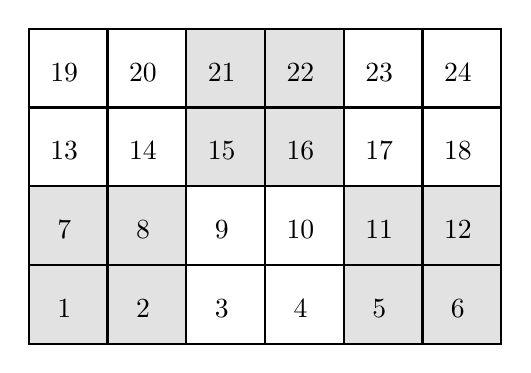
\begin{tikzpicture}
%\draw[step=0.5cm,gray,very thin] (0,0) grid (6,4); %background grid

\draw[fill=gray!23,gray!23](0,0) rectangle (2,2);
\draw[fill=gray!23,gray!23](2,2) rectangle (4,4);
\draw[fill=gray!23,gray!23](4,0) rectangle (6,2);

\draw[thick] (0,0)--(6,0)--(6,4)--(0,4)--cycle;  

\draw[thick] (0,1)--(6,1);  
\draw[thick] (0,2)--(6,2);  
\draw[thick] (0,3)--(6,3);  

\draw[thick] (1,0)--(1,4);  
\draw[thick] (2,0)--(2,4);  
\draw[thick] (3,0)--(3,4);  
\draw[thick] (4,0)--(4,4);  
\draw[thick] (5,0)--(5,4);  

\node[] at (0.45,0.45) {1};
\node[] at (1.45,0.45) {2};
\node[] at (2.45,0.45) {3};
\node[] at (3.45,0.45) {4};
\node[] at (4.45,0.45) {5};
\node[] at (5.45,0.45) {6};

\node[] at (0.45,1.45) {7};
\node[] at (1.45,1.45) {8};
\node[] at (2.45,1.45) {9};
\node[] at (3.45,1.45) {10};
\node[] at (4.45,1.45) {11};
\node[] at (5.45,1.45) {12};

\node[] at (0.45,2.45) {13};
\node[] at (1.45,2.45) {14};
\node[] at (2.45,2.45) {15};
\node[] at (3.45,2.45) {16};
\node[] at (4.45,2.45) {17};
\node[] at (5.45,2.45) {18};

\node[] at (0.45,3.45) {19};
\node[] at (1.45,3.45) {20};
\node[] at (2.45,3.45) {21};
\node[] at (3.45,3.45) {22};
\node[] at (4.45,3.45) {23};
\node[] at (5.45,3.45) {24};

\end{tikzpicture}


\end{center}

Consider now the bilinear form given by
\[
C(q^h,p^h) = \beta h \sum_{m=1}^{N_m} \sum_{i=1}^4 \int_{\partial \Omega_m}[[ q^h ]]  [[p^h ]] ds
\]
where the first summation is over all $2\times 2$ macroelements,
and the second summation runs over all inter element edges strictly within 
each macroelelement. 

The form of the stabilisation matrix $\C$ 
is similar to that above except that there is now a
local basis.

For instance, considering again element 9, it now belongs to the second macro-element
and therefore only 'sees' neighbours 4 and 9.
The resulting $\C$ matrix is shown in blue on the figure here after and 
is structure is obviously different than in the global stabilisation case, albeit 
also pentadiagonal. 


%sike90
The advantages of this local method over the global jump formulation are 
\begin{enumerate}
\item implementation is more straightforward because for assembly purposes each 2x2 block
of elements can be treated as a single macroelement \footnote{same here, not sure what they mean by this}
\item mass is conserved locally (over a macroelement), using the global jump formulation
mass is only conserved globally
\item robustness is improved in the sense that the discrete velocity solution is less sensitive 
to the magnitude of $\beta$, the influence of the stabilisation matrix being localised.
\end{enumerate}

Note also that the globally stabilised formulation corresponds to the 
extreme case of a local stabilisation based on a single macro-element \cite{grsa}.

One of the features of the local stabilisation is that if the discrete incompressibility 
constraints are added together then the jump terms sum to zero in each macro element.
Indeed, let us consider the following macro element: 

\begin{center}
\begin{flushright} {\tiny {\color{gray} (tikz\_macro.tex)}} \end{flushright}
%~~~~~~~~~~~~~~~~~~~~~~~~~~~~~~~~~~~~~~~~~~~~~~~~~~~~~~~~~~~~~~~~~~~~~~~~~~~~~~~~~~~~~~~~~~~~~~~~~~

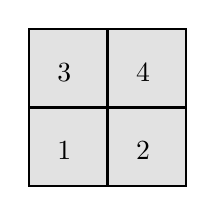
\begin{tikzpicture}
\draw[fill=gray!23,gray!23](0,0) rectangle (2,2);
\draw[thick] (0,0)--(2,0)--(2,2)--(0,2)--cycle;  
\draw[thick] (0,1)--(2,1);  
\draw[thick] (1,0)--(1,2);  
\node[] at (0.45,0.45) {1};
\node[] at (1.45,0.45) {2};
\node[] at (0.45,1.45) {3};
\node[] at (1.45,1.45) {4};
\end{tikzpicture}


\end{center}

The corresponding matrix (making abstraction of the $\beta$ term) writes:
\[
h^2
\left(
\begin{array}{cccc}
2 & -1 & -1 &0 \\
-1 & 2 & 0 & -1 \\
-1 & 0 & 2 & -1 \\
0 & -1 & -1 & 2
\end{array}
\right)
\left(
\begin{array}{c}
p_1 \\ p_2 \\ p_3 \\ p_4
\end{array}
\right)
\]
and the row/column sum of its entries is always nul.
%gresho & sani
This is crucially important to the success of the method since it implies
that the local incompressibility of the $Q_1P_0$ method is retained
after stabilisation (albeit over macro-elements).
It also suggests that a good strategy when constructing the partition 
is to form macro-elements containing as few elements as possible. 
Once a suitable macro-element partitioning has been formed, the local stabilisation
matrices can be calculated by running through the component elements, 
summing jump contributions corresponding to the internal edges. 

If one now considers the following irregular macro-element,
\begin{center}
\begin{flushright} {\tiny {\color{gray} (tikz\_macro2.tex)}} \end{flushright}
%~~~~~~~~~~~~~~~~~~~~~~~~~~~~~~~~~~~~~~~~~~~~~~~~~~~~~~~~~~~~~~~~~~~~~~~~~~~~~~~~~~~~~~~~~~~~~~~~~~


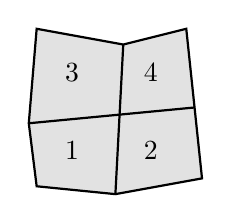
\begin{tikzpicture}
\draw[thick,fill=gray!23] (0,0)--(1,-0.1)--(2.1,0.1)--(1.9,2)--(1.1,1.8)--(0,2)--(-0.1,0.8)--cycle;  
\draw[thick] (-0.1,0.8)--(2,1);  
\draw[thick] (1,-0.1)--(1.1,1.8);  
\node[] at (0.45,0.45) {1};
\node[] at (1.45,0.45) {2};
\node[] at (0.45,1.45) {3};
\node[] at (1.45,1.45) {4};
\end{tikzpicture}




\end{center}


the corresponding matrix is given by\footnote{I suspect it should involve the normal vectors
to the edges ...?}
\[
\tilde{h}
\left(
\begin{array}{cccc}
h_{12}+h_{13} & -h_{12} & -h_{13} & 0\\
-h_{12} & h_{12}+h_{24} & 0 & -h_{24} \\
-h_{13} & 0 & h_{13}+h_{34} & -h_{34} \\
0 & -h_{24} & -h_{34} & h_{24} + h_{34}
\end{array}
\right)
\left(
\begin{array}{c}
p_1 \\ p_2 \\ p_3 \\ p_4
\end{array}
\right)
\]
where $h_{ij}$ is the length/surface of the edge betweens elements $i$ and $j$. 
The reference length $\tilde{h}$ may be computed by simply defining it to be the average 
diameter of the constituent elements. 

%grsa
In three dimensions, the 2x2x2 block is the obvious starting point for stabilising $Q_1P_0$.

Perhaps the most serious potential drawback of the local framework is that 
stability is only guaranteed if the stabilisation parameter $\beta$ is bigger than some 
critical value $\beta_0$, which needs to be estimated.

It can be estimated that $\beta=1/4$ in 2D and $\beta=1/6$ in 3D (see \cite[p636]{grsa} 
for a detailed derivation, see also \cite{vibo92}). 

%sike90
The advantages of the stabilisation procedures over the penalty method 
are especially relevant to the discretisation of 3D incompressible flow problems, 
since iterative solution methods have to be used. 
Similar stabilisation techniques to those described here are applicable to  
the three-dimensional version of the $Q_1P_0$ mixed method.

The conclusion in \cite{sike90} is as follows:
The local jump formulation proves to be an efficient method for a priori filtering of  
spurious pressure modes. It cleanly stabilises the $Q_1\times P_0$ mixed method without compromising 
its simplicity and resulting efficiency; in particular, it is very robust with respect to the magnitude
of the stabilisation parameter. 

It is reported in \cite{grsa} that when using an iterative solver, iteration counts 
are only independent of the grid in the stabilised cases: using the raw $Q_1\times P_0$ method
the iteration counts significantly increase with decreasing $h$. Note that the deterioration
of the condition number of the matrix with decreasing $h$ is worse in 3D than in 2D (but
bear in mind that one almost always use higher resolutions in 2D than in 3D, so it does not help).




A way to look at the global vs. local stabilisation schemes is presented 
on the following figure from Christon (2002) \cite{chri02}:

\begin{center}
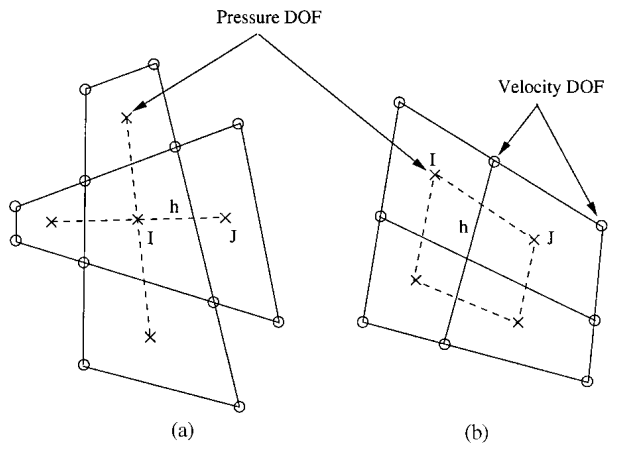
\includegraphics[width=10cm]{images/q1p0stab/chri02}\\
{\captionfont Element configuration for pressure stabilization: (a) global jump; (b) local jump.}
\end{center}

\begin{center}
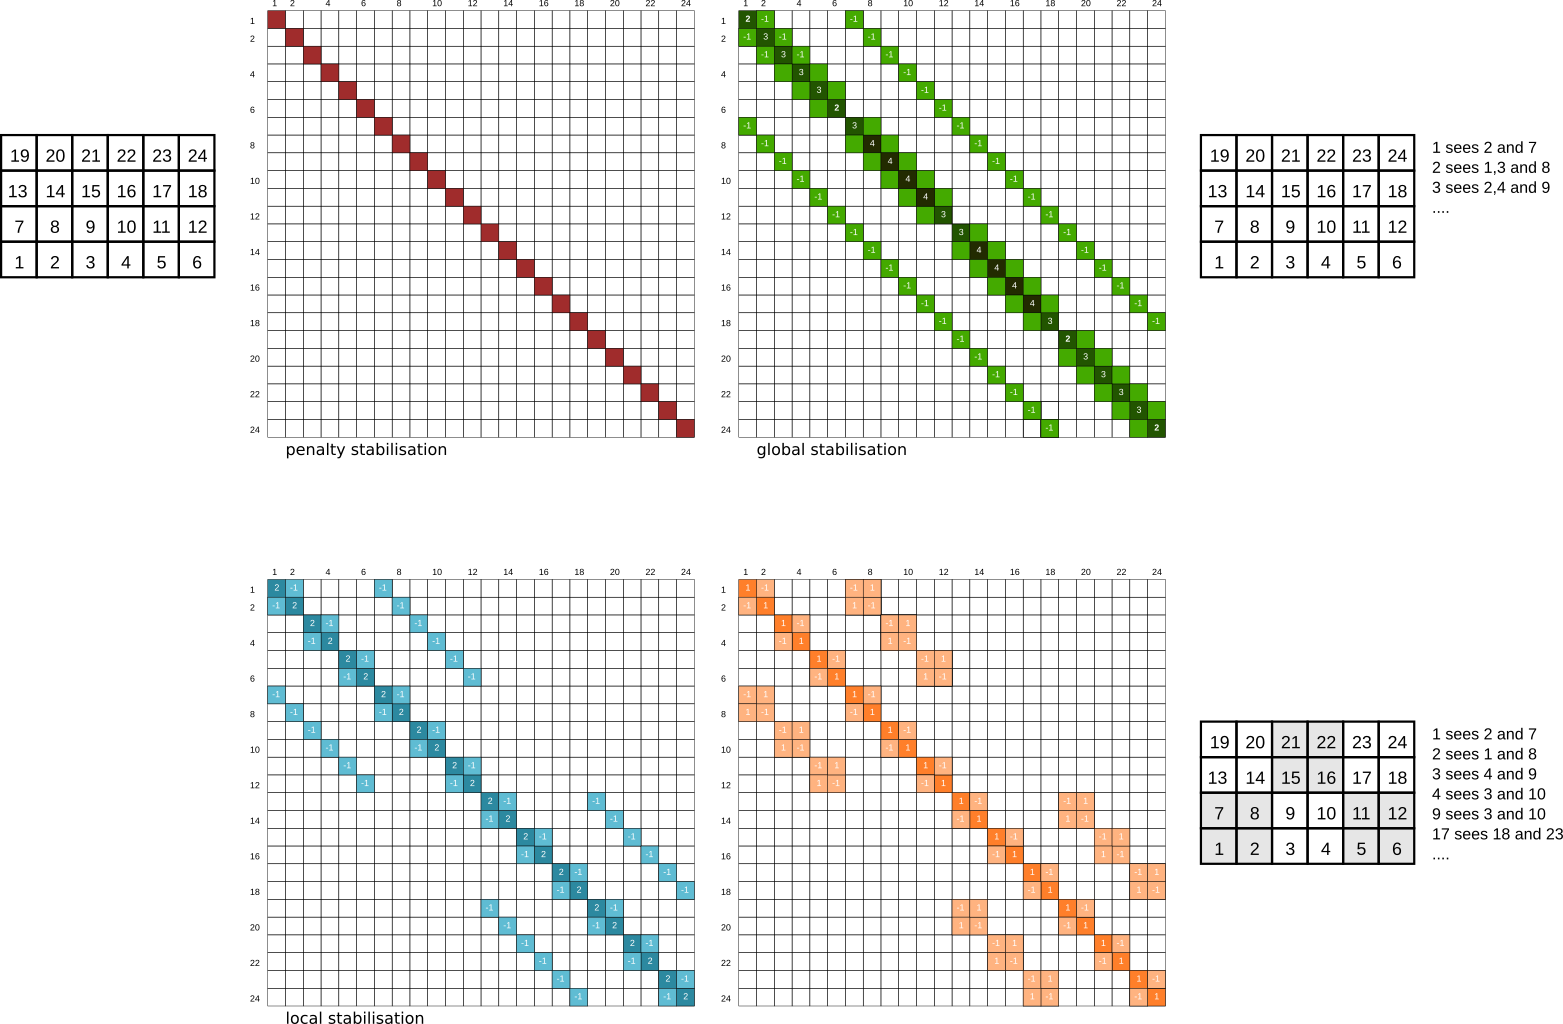
\includegraphics[width=15cm]{images/q1p0stab/stabs.png}
\end{center}


%.................................................
\paragraph{Scaling of the stabilisation matrix}

Looking at the following saddle point problem,
\[
\left( \begin{array}{cc}
\K & \G  \\ 
\G^T & -\C
\end{array} \right) \cdot
\left( \begin{array}{c}  \vec{\cal V} \\ \vec{\cal P}  \end{array} \right) = 
\left( \begin{array}{c}  \vec{f} \\ \vec{g} \end{array} \right) 
\]
where $\C$ is the stabilisation matrix,
the pressure Schur complement equation writes:

\fbox{
\parbox{6cm}{
\[
(\G^T \cdot \K^{-1} \cdot \G  + \C ) \cdot  \vec{\cal P} 
= \K^{-1}\cdot \G \cdot \vec{f} - \vec{h}
\]
}}

Dimensionless analysis: $\K \sim \eta$, $\G_{el} \sim h$, $\C \sim h^{dim}/\eta$, everything is fine.

Since the matrix $\mathbb{K}$ contains the viscosity, it is to be expected that 
the matrix $\mathbb{C}$ somehow follows the values in the $\mathbb{G}^T \mathbb{K}^{-1} \mathbb{G}$  term.
This is indeed what is advocated in Christon (2002) \cite{chri02}:
\[
\C_{ij} = \beta (\G^T\cdot \K^{-1} \cdot \G)_{ij} 
\frac{1}{\Gamma_{ij}} \int_{\Gamma_{ij}} [[\psi_i]]\;[[\psi_j]] d\Gamma
\]
where $i$ and $j$ identify adjacent elements that share a common face.
Here, $\Gamma_{ij}$ represents the shared inter-element boundary, $[[.]]$ is the jump operator,
and $\beta$ is a non-dimensional scaling parameter.
For the $Q_1\times P_0$ element, the pressure approximation is piecewise constant
with $\psi_i=1$ inside the element and zero outside.

The inclusion of the $\G^T\times \K^{-1} \cdot \G$
term (also named pressure-Poisson equation, or PPE) in the stabilisation yields proper 
dimensionality of the stabilization matrix,
accounts for scaling due to irregular elements, and still preserves the symmetry \cite{chri02}.

Note that if one wishes to compute $\C=\mathbb{G}^T \mathbb{K}^{-1} \mathbb{G}$
at the elemental level for $Q_1\times P_0$ elements, it simply boils down to a scalar,
which is rather convenient as it gives in a simple way the scaling for the
stabilisation term.

Per element, $\G_{el}=\frac{h}{2}(+1,+1-1,+1,-1,-1,+1,-1)$, which is also 
presented as Eq (4.3) in Cao (2003) \cite{cao03}, albeit in a different form.
Similarly one obtains (taking $\eta=1$):
\[
\K_{el}
=
\frac{1}{4}
\left(
\begin{array}{cccccccc}
4   & 1   & -2 & -1 & -2& -1 &0  & 1\\
1   & 4   & 1  & 0  & -1& -2 &-1 & -2\\
-2  & 1   & 4  & -1 & 0 & -1 &-2 & 1\\
-1  & 0   & -1 & 4  & 1 & -2 &1  & -2\\
-2  & -1  & 0  & 1  & 4 & 1  &-2 & -1\\
-1  & -2  & -1 & -2 & 1 & 4  &1  & 0\\
0   & -1  & -2 & 1  & -2& 1  &4  & -1\\
1   & -2  & 1  & -2 & -1& 0  &-1 & 4 \\
\end{array}
\right)
\]
Taking $\mathbb{K}_{el}^{-1}=1/diag(\mathbb{K}_{el})$, 
it is easy to (numerically) verify that (at least for square Q1P0 elements) 
the PPE simple writes $\tilde{C} = 2 h^2/\eta $.

It can be proven that the ideal value for the stabilisation parameter is given by $\beta=1/4$ \cite[p241]{elsw}.

Similar approach is taken in \cite{chsu97}

%..............................................
\paragraph{Consistency and stabilisation}


To ensure consistency it is required that  ${\bm 1}\in null(\C)$
and this precludes the use of the penalty method \cite[p239]{elsw}.

Indeed, looking at the 'red' matrix, one sees that $\mathbb{C}\cdot {\bm 1} \neq 0$
where ${\bm 1}=(1,1,1,...1)$.
Interestingly the green and blue matrices corresponding to the global and local
stabilisation schemes do verify $\mathbb{C}\cdot {\bm 1} = 0$ (the sum
of each row is strictly zero).

To provide stabilisation, it is required that
$\vec{\cal P}_\star \cdot \C \cdot \vec{\cal P}_\star > 0$ for all
spurious pressure modes $\vec{\cal P}_\star \neq 1$ in $null(\G)$ \cite[p239]{elsw}.


%..............................................
\paragraph{In three dimensions}


The matrix $\SSS$ is obtained by assembling the submatrices 
for the macroelements which, in general, are made up of 8 (i.e., 2x2x2) 
adjacent elements, as shown in the following sketch \cite{chsu97}:

\begin{center}
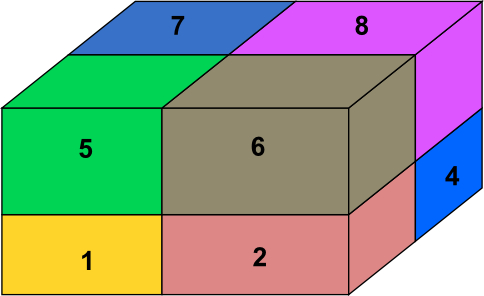
\includegraphics[width=4cm]{images/q1p0stab/macro3D}\\
{\captionfont Numbering of hexahedrons in a macroelement.\\ 
Element No. 3 is behind No. 1 and below No. 7.} 
\end{center}

For a macroelement of 8 elements as ordered in the above sketch, the submatrix is defined below:

\[
\SSS=
\left(
\begin{array}{cccccccc}
h_{12}+h_{13}+h_{h15} & -h_{12} & -h_{13} &  0  &  -h_{15} & 0  & 0 & 0 \\
-h_{21} & h_{21}+h_{24} + h_{26} & 0 & -h_{24} & 0 & -h_{26} & 0 & 0 \\
-h_{31} & ... \\
0 & ... \\
-h_{51} & ...\\
0 & ...\\
0 & ...\\
0 & ...
\end{array}
\right)
\]
in which $h_{ij}$ is the length scale for elements ‘i’ and ‘j’ in the macroelement. 
The matrix $\SSS$ is symmetric, since $h_{ij}=h_{ji}$. 

Two approaches are possible  for computing the length scale $h_{ij}$:
\begin{itemize}
\item the square root of the interior inter-element surface area between elements ‘i’ and ‘j’
\item the quotient of the interior inter-element surface area divided by the cube 
root of the average element volume of the macroelement.
\end{itemize}


%.............................................................................
\paragraph{The stabilisation matrix in the presence of viscosity contrasts}

The previously advocated scaling of the $\C$ matrix is not clear when it comes to viscosity contrasts
from one element to the other. When using a Conjugate Gradient method for the outer iterations, 
the matrix $\C$ must be SPD. However, scaling the row entries of the $\C$ matrix by the element 
viscosity still yields a structurally symmetric matrix, but not a numerically symmetric one !
Some form of viscosity averaging must then take place between adjacent elements so that the contribution 
from elt A to B in exactly the same as B to A.  

However, in order for the stabilisation to remain consistent (FIND SOURCE) it must 
satisfy $\C\cdot \vec{1}= 0$, 
i.e. it should have zero effect on a constant pressure field, which simply forces
the sum of the entries for each row to be nul. This requirement makes the above viscosity averaging 
idea very difficult in practice in the global case (satisfying both symmetry and consistency).

In the global stabilisation case, a reference viscosity valid for the whole domain should be used. 

In the local stabilisation approach, each macro-element is 'isolated' from the others so that an average
viscosity can be computed for each block of 4 (2D) or 8 (3D) elements and used to scale the $\C$ matrix
yielding a symmetric matrix and a consistent one too.
Let us look at the following patch of elements. Each macro-element is assigned an average viscosity
(represented by a different colour for each), 
function of the elemental viscosities within the macro-element. 

\begin{center}
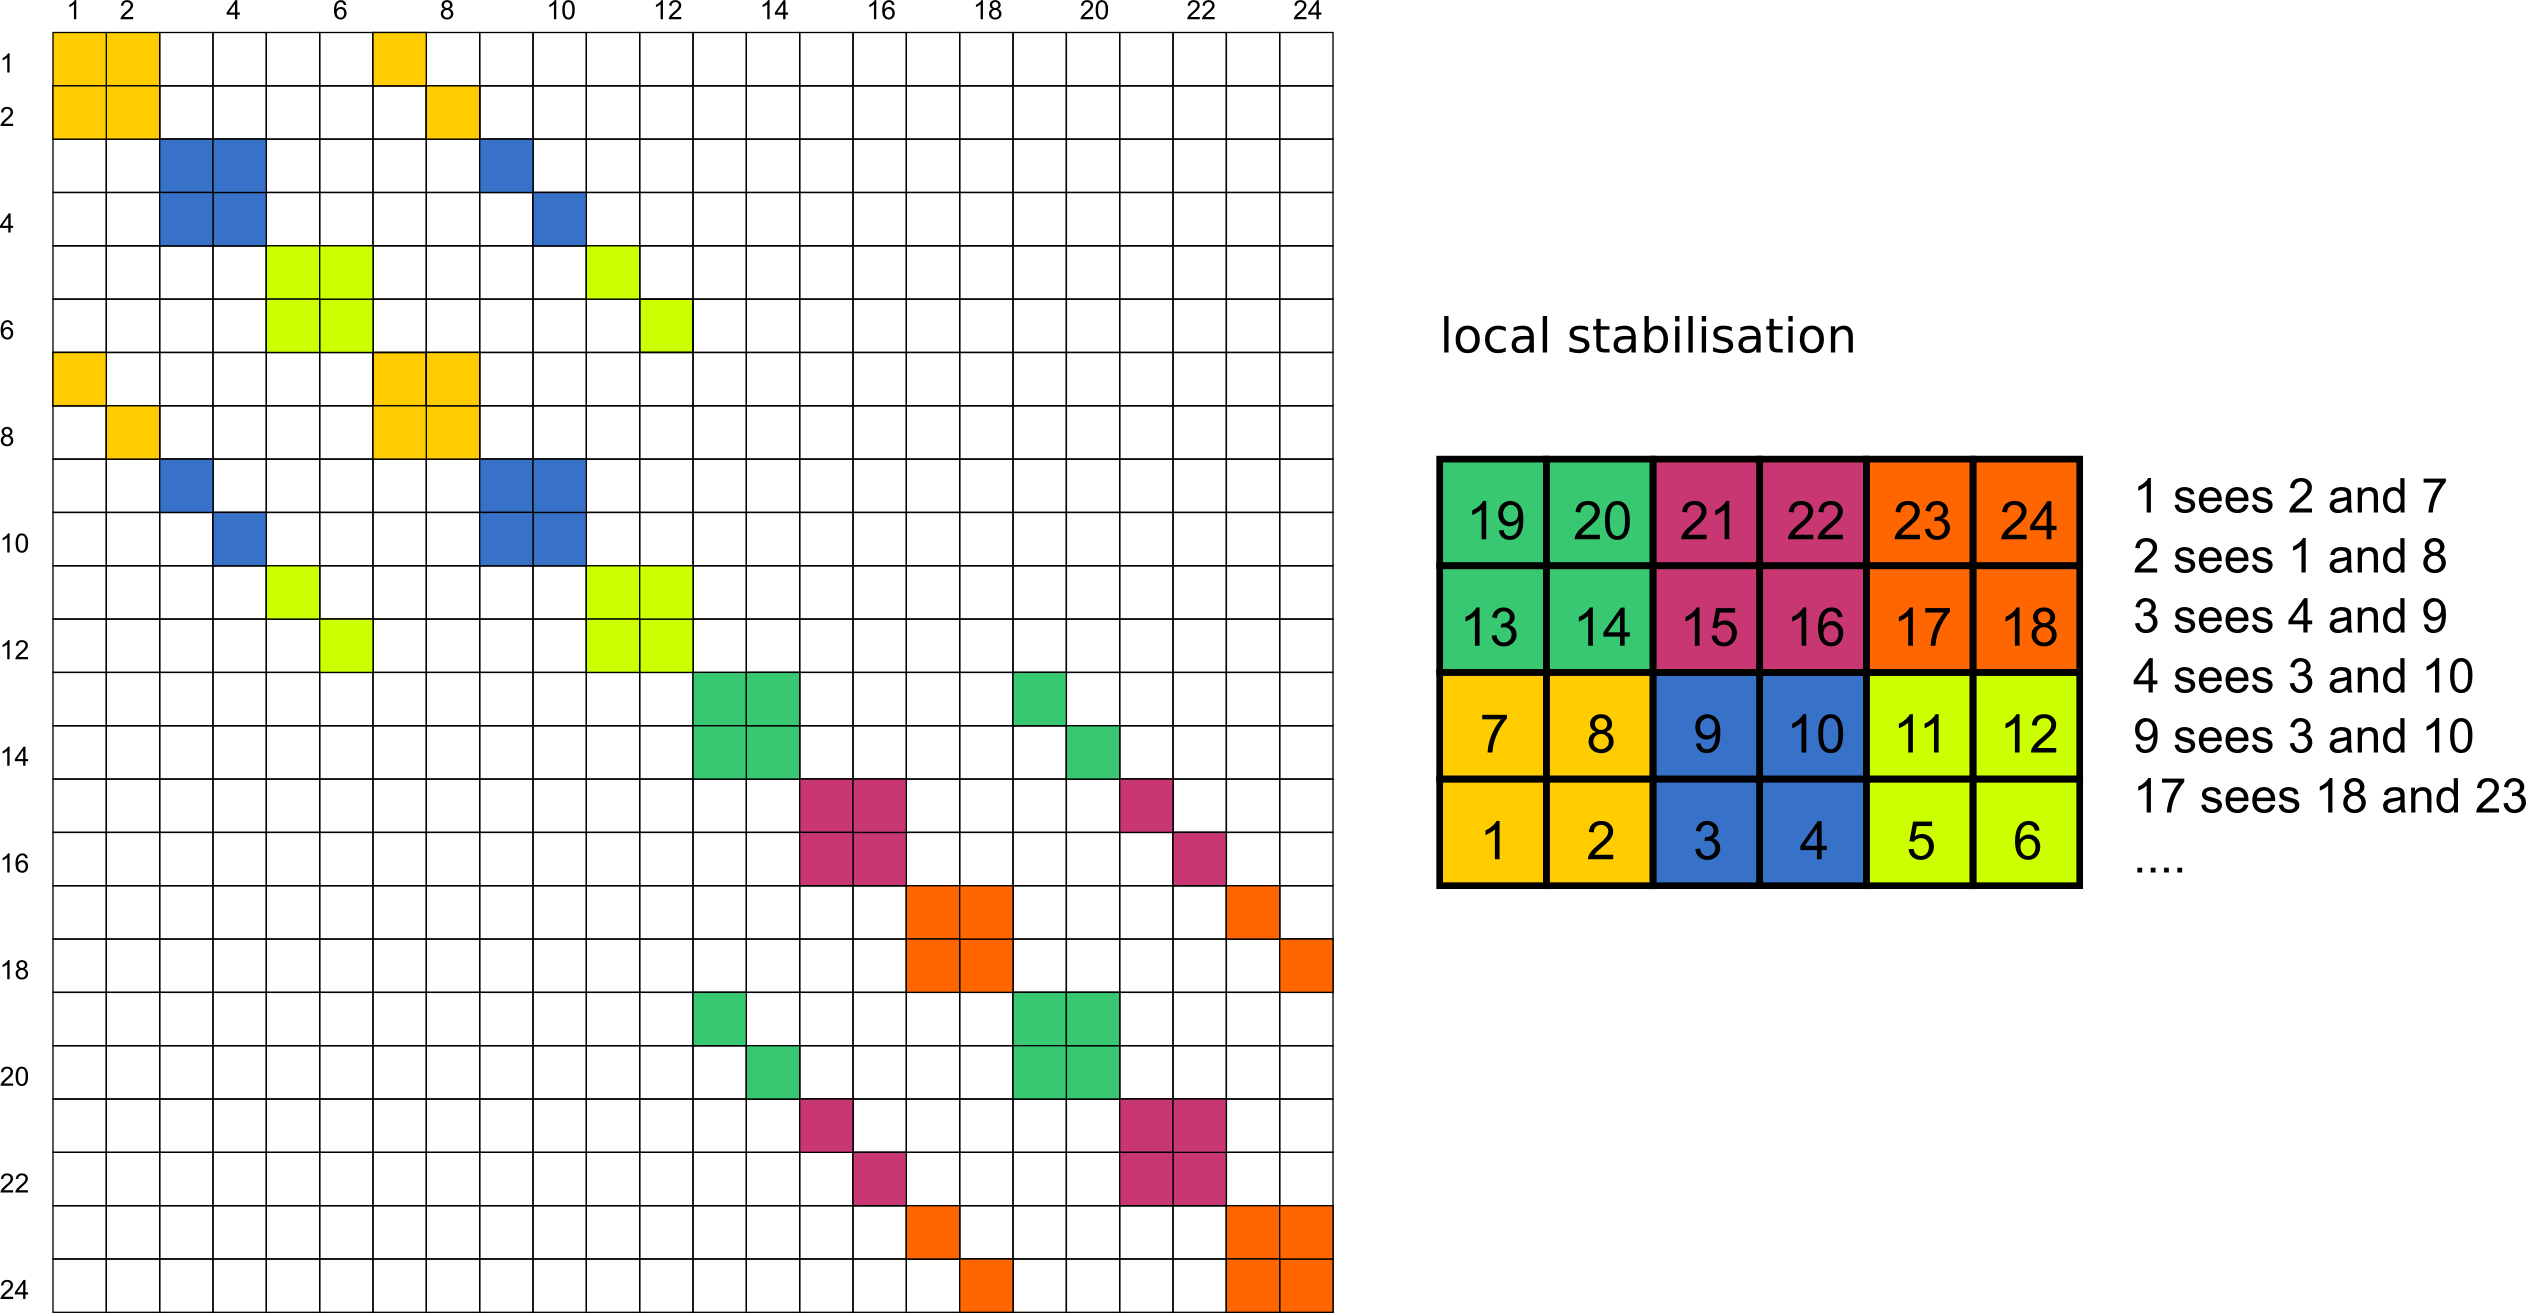
\includegraphics[width=15cm]{images/q1p0stab/stab_local.png}
\end{center}

In the matrix $\C$ the nonzero values are also shown with the corresponding colours.
The matrix symmetry is preserved: elt 1 sees 2 and vice versa, but the prefactor is the same, corresponding
to the yellow colour. Each row of the matrix contains only one colour, thereby preserving consistency.
 
REMARK: I suspect the matrix is still SPD as it is the previous matrix multiplied by a diagonal matrix.



This approach is now abandonned. The solution (or at least) the inspiration came from Christon (2002) \cite{chri02}.The author gives his recipe to scale the $\C$ matrix:

\begin{center}
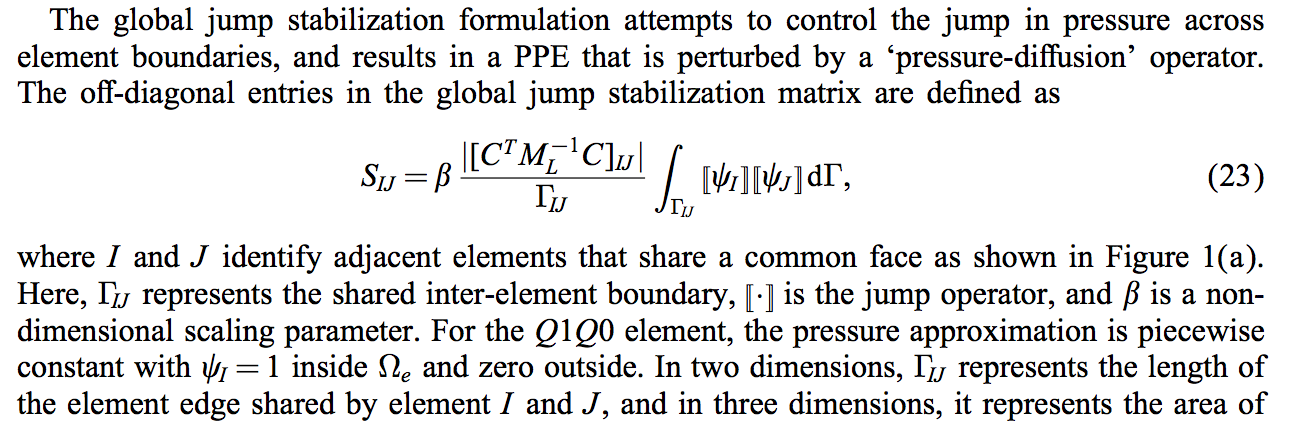
\includegraphics[width=15cm]{images/q1p0stab/chri_a.png}\\
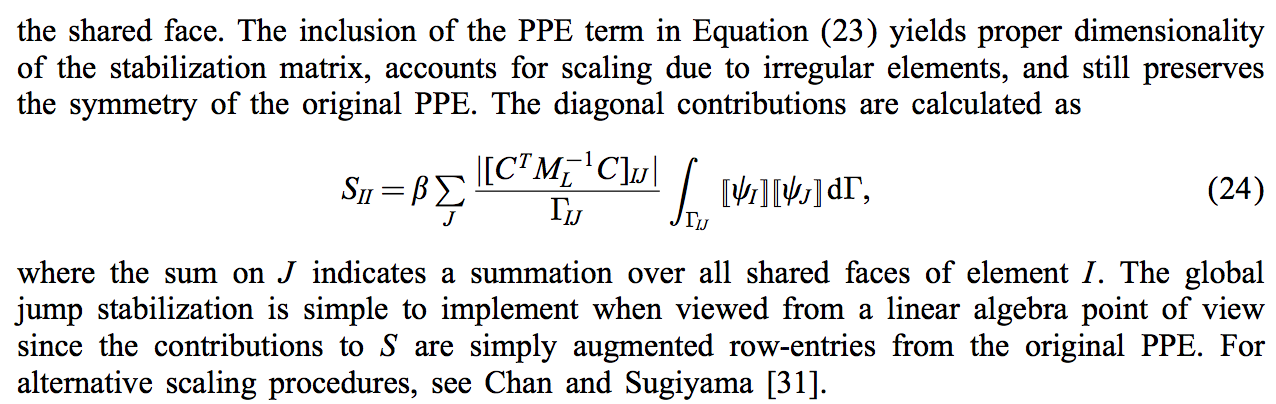
\includegraphics[width=15cm]{images/q1p0stab/chri_b.png}
\end{center}

I however find this method unpractical because one needs to compute the
Schur complement $\G^T \K^{-1} \G$ (or $C^T M_L^{-1} C$ in his case).
I suspect he does not really build it but he remains evasive on his 
workaround. 
I need to find an approximate expression. I first replace $\K$ by
its diagonal $\K_d$: $\G^T \K_d^{-1} \G$. The diagonal contains 
positive terms proportional to the dynamic viscosity. Its inverse 
is simply a diagonal matrix containing the inverse of the terms.
One can therefore write: 
\begin{eqnarray}
\G^T \K_d^{-1} \G 
&=& \G^T \sqrt{\K_d}^{-1} \sqrt{\K_d}^{-1} \G  \nn\\
&=& ( \sqrt{\K_d}^{-1} \G)^T (\sqrt{\K_d}^{-1} \G)  \nn\\
\end{eqnarray}

We know that $\G \sim h$ (in amplitude) and that $\K \sim \mu$ so that
$ \G^T \K_d^{-1} \G \sim h^2/\mu$. 
The $(IJ)$ component of this matrix will then be approximated by
$(\G^T \K_d^{-1} \G)_{IJ} \sim  h^2/\sqrt{\mu_I \mu_J} $. 
This has the added benefit that it yields a symmetric matrix too
(the $IJ$ component is equal to the $JI$ component).
However, there is no guarantee of consistency (i.e. the sum of the
terms on a row do not necessarily add up to zero). 
Diagonal terms are therefore computed as in Eq. (24) of \cite{chri02}.





%--------------------------------------------------------------------------------------------------
\subsubsection{The stabilised bi/tri-linear velocity - bi/tri-linear pressure element ($Q_1\times Q_1$-stab)}
\label{ss:pairq1q1stab}
\begin{flushright} {\tiny {\color{gray} pair\_q1q1stab.tex}} \end{flushright}
%~~~~~~~~~~~~~~~~~~~~~~~~~~~~~~~~~~~~~~~~~~~~~~~~~~~~~~~~~~~~~~~~~~~~~~~~~~~~~~~~~~~~~~~~~~~~~~~~~~

\begin{minipage}[t]{0.5\textwidth}

\begin{center}
\begin{tikzpicture}
%\draw[fill=gray!23,gray!23](0,0) rectangle (5,5);
%\draw[step=0.5cm,gray,very thin] (0,0) grid (4,4); %background grid
\draw[thick] (1,1) -- (3,1.2) -- (2.7,3) -- (1.1,3.1) -- cycle;  
\node[] at (0.8,0.8) {0};
\node[] at (3.2,1)   {1};
\node[] at (2.9,3.1) {2};
\node[] at (0.9,3.2) {3};
\draw[black,fill=teal] (1,1)     circle (2pt); \draw[violet] (1,1) circle (4pt);
\draw[black,fill=teal] (3,1.2)   circle (2pt); \draw[violet] (3,1.2) circle (4pt);
\draw[black,fill=teal] (2.7,3)   circle (2pt); \draw[violet] (2.7,3) circle (4pt);
\draw[black,fill=teal] (1.1,3.1) circle (2pt); \draw[violet] (1.1,3.1) circle (4pt);
\draw[black,fill=teal] (3.1,0.2) circle (2pt); 
\node[] at (3.4,0.2) {$\vec\upnu$};
\draw[violet] (4.1,0.2) circle (4pt); 
\node[] at (4.4,0.2) {$p$};
\node[] at (2.5,4.5) {4 vel. nodes, 4 press. nodes};
\end{tikzpicture}\\
\end{center}

\end{minipage}
\begin{minipage}[t]{0.5\textwidth}

\begin{center}
\begin{tikzpicture}
\draw[fill=gray!23,gray!23](0,0) rectangle (5,5);
%\draw[step=0.25cm,gray,very thin] (0,0) grid (5,4); %background grid
\draw[thick] (1,0.5) -- (3.25,0.75) -- (3,3) -- (0.5,2.5) -- cycle; %1-2-6-5
\draw[thick] (3.25,0.75) -- (4,1.5) -- (4.25,3.75) -- (3,3) -- cycle; %2-3-7-6
\draw[thick] (0.5,2.5) -- (3,3) -- (4.25,3.75) -- (1.75,3.5) -- cycle; %5-6-7-4
\draw[thin]   (1,0.5) -- (2,1.75) -- (1.75,3.5) -- (0.5,2.5)   --cycle; % 1-0-4-5 
\draw[thin] (2,1.75) -- (4,1.5); 
%\node[] at (0.8,0.8) {0};
%\node[] at (3.2,1) {1};
%\node[] at (2.9,3.1) {2};
%\node[] at (0.9,3.2) {3};
\draw (1,0.5) circle (4pt);
\draw (3.25,0.75) circle (4pt);
\draw (4,1.5) circle (4pt);
\draw (2,1.75) circle (4pt);
\draw (0.5,2.5) circle (4pt);
\draw (3,3) circle (4pt);
\draw (4.25,3.75) circle (4pt);
\draw (1.75,3.5) circle (4pt);
\draw[black,fill=black] (1,0.5)   circle (2pt);
\draw[black,fill=black] (3.25,0.75)   circle (2pt);
\draw[black,fill=black] (3,3)   circle (2pt);
\draw[black,fill=black] (0.5,2.5)   circle (2pt);
\draw[black,fill=black] (1.75,3.5)  circle (2pt);
\draw[black,fill=black] (4.25,3.75)  circle (2pt);
\draw[black,fill=black] (4,1.5) circle (2pt);
\draw[black,fill=black] (2,1.75) circle (2pt);
\draw[black,fill=black] (3.1,0.2) circle (2pt); \node[] at (3.4,0.2) {$\vec\upnu$};
\draw (4.1,0.2) circle (4pt); \node[] at (4.4,0.2) {$p$};
\node[] at (2.5,4.5) {8 vel. nodes, 8 press. nodes};
\end{tikzpicture}\\
\end{center}

\end{minipage}

The ${\bm Q}_1\times Q_1$ element is not LBB-stable but it can be stabilised. Despite
some applications in geodynamics (it is used in \textcite{bugs09} (2009) 
and \textcite{busa13} (2013)), it is not appropriate for buoyancy-driven flows, 
as shown in \textcite{thba22}.

See \textcite{nosi01} (2001) for a fourier analysis of the normal 
and stablised (a la \textcite{hufb86} (1986)) ${\bm Q}_1\times Q_1$ element.
Stabilisation is worked out out in \textcite{dobo04} (2004), \textcite{bodg06} (2006), 
and \textcite{bodo06} (2006).

\begin{itemize}
\item 
${\bm Q}_1\times P_0$-stab. Pro: stabilisation can be switched off; Con: stabilisation for deformed elements? 
problem near boundaries: incomplete stencil? choice of parameter $\beta$.
\item 
${\bm Q}_1\times Q_1$-stab. Pro: easier to implement than ${\bm Q}_1\times P_0$-stab, stabilisation local to element, 
easier when elements are not rectangular, no free parameter; Con: stabilisation cannot be switched off.
\end{itemize}

\Literature: \textcite{shry78,temr92,tezd92,grcc95,idsn95,knto00,fros07,lihc09}. 
See \textcite{brlu09} for a review of local projection stabilisation for incompressible flow problems. 

This unstable pair is also used in ice sheet modelling \textcite{heah18} , \textcite{zhjg11}, 
\textcite{zwgg07}. A ${\bm P}_1\times P_1$ version of it is used in \textcite{kahp20} (2020).






%-----------------------------------------------------------------
\subsubsection{The Rannacher-Turek element - rotated ${ Q}_1\times P_0$} \label{ss:RTq1p0}

This element is the natural quadrilateral analogue
of the well-known triangular $P_1^{nc} $Stokes element of Crouzeix-Raviart \cite{crra73}.
This element is sometimes called $Q_1^{rot} \times Q_0$ or the Rannacher-Turek element 
\cite[Section 3.6.5]{john16} (see also Appendix~B.4, example B.53 of \textcite{john16}).
This rectangular nonconforming \cite{crfa89} element is termed the rotated $Q_1$ element 
because of the fact that $r^2-s^2$ can be generated from $rs$ (occurring in the bilinear $Q_1$ 
element) by a rotation of 45$\degree$ \cite[p93]{chen}.
The velocity approximation is achieved by rotated dim-linear functions that have 
continuous degrees of freedom on
the faces of the mesh cells as we have seen in Section~\ref{ss:rq1}.
This element was introduced in Rannacher \& Turek (1992) \cite{ratu92} 
has been proven to satisfy the inf-sup condition. It has been studied comprehensively in Schieweck 
(1997)\footnote{Habilitation thesis in German}, \cite{shzh06} and in Turek \cite{ture94,ture96}.
Superconvergence properties have also been reported \cite{misx06,misx07}.
It has been used in 2D \cite{maky17} and 3D \cite{klll96,gekm08} and forms the basis of the FeatFlow 
software\footnote{\url{http://www.featflow.de/en/index.html}}. 
It is used in the PhD thesis of Gastaldo \cite{gast07} and Ouazzi \cite{ouaz05}.
It has been 
successfully coupled to multigrid solvers \cite{chos98,tuos02}.
This element has been compared to the stabilised $Q_1\times P_0$ element \cite{lisi13}.
It is mentioned in \cite{hans11}

It essentially comes in two flavours, the Middle Point (MP) and the Mid Value (MV) one.

\begin{remark} 
John \cite{john16} explains that: "For the point-value-oriented non-conforming finite element spaces (MP), 
the value of the Dirichlet boundary
condition in the barycenter of the faces at the boundary is taken. Using the mean-
value-oriented spaces (MV), one computes the integrals of the boundary condition on
these faces and normalizes with the area of the faces to set the boundary values.
In the case of homogeneous Dirichlet boundary conditions, the boundary values
computed in both ways are zero."
\end{remark}

\begin{remark} 
John also makes a very important point: "There are also unmapped (non-parametric) versions of 
these finite element spaces, which define the polynomials directly on the mesh cell K. It is shown in Rannacher
and Turek (1992) \cite{ratu92} that these versions are inf-sup stable on more general meshes than
the mapped (parametric) version of the $Q_1^{rot}\times Q_0$ finite element, e.g., on strongly
nonuniform meshes. Considering all four types of $Q_1^{rot}\times Q_0$ finite elements, the
optimal order of convergence on perturbed meshes is achieved only by the mean-
value-oriented version of the unmapped $Q_1^{rot}\times Q_0$   finite element.
\end{remark}

Mahmood \etal \cite{maky17} mention a very important fact: "The chosen nonconforming element requires
additional stabilization for handling the deformation tensor formulation due to missing Korn's inequality 
\cite{horg95,knob00}.
To this end we employ the standard edge oriented stabilization \cite{tuos02,tuou07} in our simulations."
This is a rather unfortunate fact that although LBB stable this element needs an additional 
term in the weak form (see Turek \etal (2002) \cite{tuos02}) 
so as to suppress parasitic velocity modes when the div-grad formulation 
of the Stokes equation is used (as opposed to the Laplace formulation -- see \cite[Section 6.5.2]{dohu03}).

\Literature \textcite{shee20} (2020), \textcite{chen92} (1992) , \textcite{chen93} (1993) 








%------------------------------------------------------------------
\subsubsection{The ${ P}_1\times P_0$ pair} \label{ss:p1p0}

$P_1\times P_0$: example 3.70 in \textcite{john16} (book),
\index{general}{$P_1\times P_0$}


Elman Silvester Wathen say (5.3.3) that 
``it can be readily stabilized using the pressure jump
stabilization together with an appropriate macroelement subdivision.'' 

\textcite{qizh07b} (2007) states: ``the element is unstable for any mesh since
the dimension of the discrete velocity space is always less than that of the pressure space (with
Dirichlet boundary condition).'' The authors explain a filter algorithm to make the
element usable. 

\textcite{arno93} (1993) states: ''Unfortunately, this simplest possible Stokes element is notoriously unstable. On any tri-
angulation with at least three vertices on the boundary the dimension of the pressure
space exceeds that of the velocity space [...] and the finite
dimensional problem is singular. 
Moreover, while the discrete velocity field $u_h$ is uniquely
determined (as it is for any conforming method for the Stokes problem), for this choice of
elements $u_h$ belongs to the space of divergence-free fields piecewise linear fields, and on
many meshes, for example on a uniform diagonal mesh of the square [...],
this space is known to reduce to zero. So even after accounting for the indeterminancy of
the pressure we have no convergence.''

Example 3.2 of \textcite{bobf08} (2008) explains neatly the locking phenomenon and how 
to circumvent it via a so-called cross-grid macroelement.

I have not found a paper yet which showcases its accuracy on a mms and compares it to other 
element pairs.




%------------------------------------------------------------------
\subsubsection{The ${ P}_2\times P_0$ pair} \label{ss:p2p0}
 \cite{bobf08}, \cite{cakp18} stable (Kanschat book)

compared with P1NC-P0 and BR element in \textcite{cakp15} (2015).


%------------------------------------------------------------------
\subsubsection{The ${ Q}_2\times Q_0$ pair} \label{ss:pairq2q0}
\index{general}{${\bm Q}_2 \times Q_0$}

Quadratic velocities, constant pressure. The element satisfies the inf-sup condition, 
but the constant pressure assumption may require fine discretisation.
source?


%------------------------------------------------------------------
\subsubsection{The ${ P}_1\times P_1$-stabilised pair} \label{ss:P1P1stab}

Like its quadrilateral counterpart ${\bm Q}_1\times Q_1$, the 
$P_1\times P_1$ pair is not stable and needs to be stabilised \cite{nosi98,tasu00}.
TerraNeo code uses stabilised with PSPG \cite{babd20}.

\textcite{nosi98}

%--------------------------------------------------------------------------------------------------
\subsubsection{The ${ P}_1^+\times P_1$ (MINI) pair in 2D \& 3D \label{pair:mini}}
\begin{flushright} {\tiny {\color{gray} pair\_mini.tex}} \end{flushright}
%~~~~~~~~~~~~~~~~~~~~~~~~~~~~~~~~~~~~~~~~~~~~~~~~~~~~~~~~~~~~~~~~~~~~~~~~~~~~~~~~~~~~~~~~~~~~~~~~~~

\noindent
\begin{minipage}{0.48\textwidth}
The \index{general}{MINI element} MINI element was first introduced in Arnold \etal, 1984 \cite{arbf84}.
It is also discussed in section 3.6.1 of John \cite{john16}.


As explained in Braess \cite{braess}, since the support of the bubble is restricted to the element, 
the associated variable (dofs living on the bubble) can be eliminated from the resulting 
system of linear equations by static condensation. \index{general}{Static Condensation}
Also, the MINI element is cheaper than the Taylor-Hood element but it is commonly accepted
that it yields a poorer approximation of the pressure.
\end{minipage}\hfill
\begin{minipage}{0.48\textwidth}
\begin{flushright} {\tiny {\color{gray} (tikz\_mini.tex)}} \end{flushright}
%~~~~~~~~~~~~~~~~~~~~~~~~~~~~~~~~~~~~~~~~~~~~~~~~~~~~~~~~~~~~~~~~~~~~~~~~~~~~~~~~~~~~~~~~~~~~~~~~~~

\begin{center}
\begin{tikzpicture}
%\draw[fill=gray!23,gray!23](0,0) rectangle (5,5);
%\draw[step=0.5cm,gray,very thin] (0,0) grid (5,3.5); %background grid
\draw[thick] (1,0.5) -- (4,1)  -- (3,3) -- cycle; %1-9-2-6-5

%pressure nodes
\draw[violet] (1,0.5) circle (4pt); % 0 
\draw[violet] (4,1) circle (4pt); % 1 
\draw[violet] (3,3) circle (4pt); % 2 

%velocity nodes
\draw[black,fill=teal] (1,0.5)   circle (2pt);
\draw[black,fill=teal] (4,1)   circle (2pt);
\draw[black,fill=teal] (3,3)   circle (2pt);
\draw[black,fill=teal] (2.75,1.5)   circle (2pt);

% legend
\draw[black,fill=teal] (3.1,0.2) circle (2pt); \node[] at (3.4,0.2) {$\vec\upnu$};
\draw[violet] (4.1,0.2) circle (4pt); 
\node[] at (4.4,0.2) {$p$};
\node[] at (2.5,3.75) {4 vel. nodes, 3 press. nodes};
\end{tikzpicture}\\
\end{center}


\end{minipage}

\begin{remark}
Note that Franca \& Oliveira (2003) \cite{frol03} propose an equal-order-linear-continuous 
velocity-pressure variables which is enriched 
with velocity {\it and} pressure bubble functions to model the Stokes problem. 
They show by static condensation that
these bubble functions give rise to a stabilized method involving least-squares forms of 
the momentum and of the
continuity equations. In some cases their approach recovers 
the MINI element. Also check Ganesan \etal (2008) \cite{gamt08}.
\end{remark}


The 3D MINI element is not very common but it is used for instance in Pichelin \& Coupez (1998) 
\cite{pico98}. It is also said to be LBB stable in Reddy \cite[p180]{reddybook2}.

\begin{center}
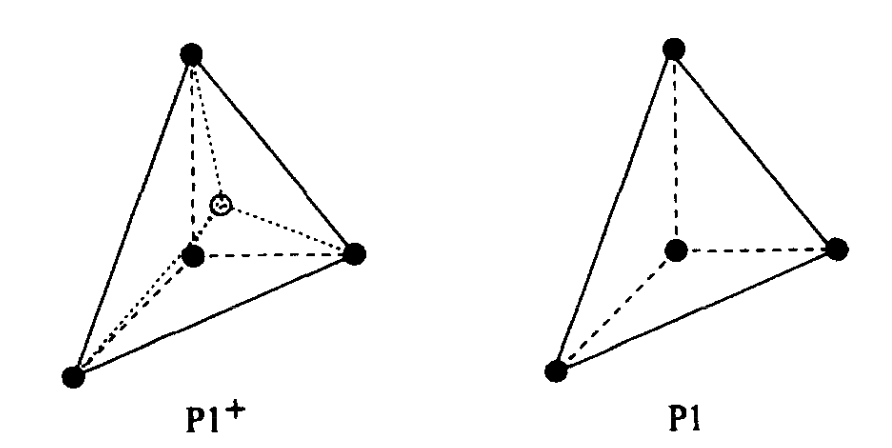
\includegraphics[width=8cm]{images/mini/mini3D}\\
{\captionfont Velocity and pressure nodes for the 3D MINI element, taken from \cite{pico98}}
\end{center}

Note that this element is used in Braess \& Wriggers (2000) \cite{brwr00} 
in the context of Arbitrary Lagrangian Eulerian 
finite element analysis of free surface flows, and also 
in Zlotnik \etal (2007) \cite{zldf07} for subduction with X-FEM technique. 
\index{general}{X-FEM}


%--------------------------------------------------------------------------------------------------
\subsubsection{The ${ P}_2\times P_1$ pair \label{ss:p2p1}}
\begin{flushright} {\tiny {\color{gray} pair\_p2p1.tex}} \end{flushright}
%~~~~~~~~~~~~~~~~~~~~~~~~~~~~~~~~~~~~~~~~~~~~~~~~~~~~~~~~~~~~~~~~~~~~~~~~~~~~~~~~~~~~~~~~~~~~~~~~~~

\noindent
\begin{minipage}{0.54\textwidth}
From Segal \cite{segal}: \say{Taylor-Hood elements \cite{taho73} 
are characterized by the fact that the pressure is continuous in the region $\Omega$. 
A typical example is the quadratic triangle (${\bm P}_2\times P_1$ element).
In this element the velocity is approximated by a quadratic polynomial and the pressure by a
linear polynomial. One can easily verify that both approximations are continuous over 
the element boundaries.}

It can be shown, Segal (1979), that this element is admissible if at least 3 elements 
are used. The quadrilateral counterpart of this triangle is the ${\bm Q}_2\times Q_1$ element.
Reddy and Gartling \cite[p179]{reddybook2} also report this element to be LBB stable.
It is also mentioned in \textcite{nath93}.

\Literature: Schubert \& Anderson \cite{scan85}, Leng \etal \cite{lejx14}, Cuffaro \etal \cite{cump20}
\end{minipage}
\hfill
\begin{minipage}{0.42\textwidth}
\begin{center}
\begin{flushright} {\tiny {\color{gray} (tikz\_p2p1.tex)}} \end{flushright}
%~~~~~~~~~~~~~~~~~~~~~~~~~~~~~~~~~~~~~~~~~~~~~~~~~~~~~~~~~~~~~~~~~~~~~~~~~~~~~~~~~~~~~~~~~~~~~~~~~~

%\begin{center}
\begin{tikzpicture}
%\draw[fill=gray!23,gray!23](0,0) rectangle (5,5);
%\draw[step=0.5cm,gray,very thin] (0,0) grid (5,3.5); %background grid
\draw[thick] (1,0.5) -- (4,1)  -- (3,3) -- cycle; %1-9-2-6-5

%pressure nodes
\draw[violet] (1,0.5) circle (4pt); % 0 
\draw[violet] (4,1) circle (4pt); % 1 
\draw[violet] (3,3) circle (4pt); % 2 

%velocity nodes
\draw[black,fill=teal] (1,0.5)   circle (2pt);
\draw[black,fill=teal] (4,1)   circle (2pt);
\draw[black,fill=teal] (3,3)   circle (2pt);

\draw[black,fill=teal] (2.5,0.75)   circle (2pt);
\draw[black,fill=teal] (2,1.75)   circle (2pt);
\draw[black,fill=teal] (3.5,2)   circle (2pt);

% legend
\draw[black,fill=teal] (3.1,0.2) circle (2pt); \node[] at (3.4,0.2) {$\vec\upnu$};
\draw[violet] (4.1,0.2) circle (4pt); 
\node[] at (4.4,0.2) {$p$};
\node[] at (2.5,3.75) {6 vel. nodes, 3 press. nodes};
\end{tikzpicture}
%\end{center}


\end{center}
\end{minipage}






%----------------------------------------------------------------------
\subsubsection{The ${ P}_2^+\times P_{-1}$ pair  (Crouzeix-Raviart) }
\label{sec:crouzeix-raviart}
\begin{flushright} {\tiny {\color{gray} pair\_crouzeixraviart.tex}} \end{flushright}
%~~~~~~~~~~~~~~~~~~~~~~~~~~~~~~~~~~~~~~~~~~~~~~~~~~~~~~~~~~~~~~~~~~~~~~~~~~~~~~~~~~~~~~~~~~~~~~~~~~

Since the $P_2\times P_{-1}$ pair is not LBB stable \cite[p179]{reddybook2}, 
(see also table 3.13-1 of \textcite{grsa})
it is enhanced by a cubic bubble and is therefore called $P_2^+\times P_{-1}$. 

This element was first introduced in \cite{crra73}.
It is the element used in the MILAMIN code \cite{daks08}.
It is a seven-node triangle with quadratic velocity shape 
functions enhanced by a cubic bubble function and discontinuous linear interpolation for 
the pressure field \cite{cuss86}. 
This element is LBB stable and no additional stabilization techniques are required\cite{elsw}.
The '+' in its name stands for the bubble while the '-' stands for the discontinuous
character of the pressure field: once again, it is $P_1$ over the element, but discontinuous
across element edges.

\begin{remark}
Cuvelier \etal, 1986 \cite{cuss86} recommend a 6-point or 7-point quadrature rule for this element.
\end{remark}

\begin{remark}
Segal \cite{segal} explains 
for output purposes (printing, plotting etc.) the discontinuous pressures are averaged 
in vertices for all the adjoining elements. See also Fig. 7.3 of \cite{cuss86}.
\end{remark}

\begin{remark}
The simplest Crouzeix-Raviart element is the non-conforming linear triangle 
with constant pressure \cite{cuss86}, see Section~\ref{ss:p1ncp0}.
\end{remark}

It is worth noting that this element has more degrees of freedom  than the 
Taylor-Hood element for the same order of accuracy. However, since the 
bubble can be eliminated, one can design a modified version of this element.
\todo[inline]{Check Cuvelier book chapter 8 for modified element}

\begin{remark}
I have once asked the (main) author of MILAMIN why he chose this element, for 
example over the $P_2\times P_1$. His answer is as follows:
"Elements with continuous pressure  are incapable of converging in the Linf 
norm for mechanical problems exhibiting pressure jumps such as the inclusion-host setup. 
During my MSc and PhD I was focusing on sharp heterogeneities, so this is why I decided 
to choose $P_2^+\times P_{-1}$. 
You will see that it is also easy to invert the pressure mass matrix for such elements, 
which is really useful (both for the augmentation and preconditioning)."
\end{remark}

This element is used by Poliakov and Podlachikov \cite{popo92} to study the deformation of 
the surface above a rising diapir. Note that they actually use a 
``13 point integration formula (Hughes 1987) for calculation of the stiffness matrix was 
used in order t o conserve detailed information from the marker field in the coarse FEM mesh''. 
It is also used in \cite{anmp15} in the context of a new free-surface stabilization scheme. 
It is the element used in LaCoDe \cite{demh19}.
It is mentioned in Section~6.2 in \textcite{bobf08} (2008).



%----------------------------------------------------------------------
\subsubsection{The ${ P}_2^+\times P_{1}$ pair \label{ss:p2pp1}}

This element pair is not to be mistaken for the Crouzeix-Raviart. Both share the same $P_2^+$ space
for the velocity but this element has a continuous linear pressure.  
It is mentioned in Table~3.13-1 of \textcite{grsa}: ``LBB stable. Second order. cubic bubble. good element''.

Implemented in \stone~120.


%------------------------------------------------------------------
\subsubsection{The ${ P}_2\times (P_1+P_0)$ pair} \label{ss:p2p1p0}
\begin{flushright} {\tiny {\color{gray} pair\_p2p1p0.tex}} \end{flushright}
%~~~~~~~~~~~~~~~~~~~~~~~~~~~~~~~~~~~~~~~~~~~~~~~~~~~~~~~~~~~~~~~~~~~~~~~~~~~~~~~~~~~~~~~~~~~~~~~~~~

This element pair is discussed in 5.3.3 of Elman, Silvester and Wathen: 

``[Another] possibility is to construct a hybrid pressure approximation by 
combining the continuous linear pressure approximation with the discontinuous constant pres-
sure approximation. The resulting mixed method is referred to as the $P_2-P_{-1*}$ 
approximation and enjoys the best of both worlds; it has locally 
incompressibility, and yet it does not have its accuracy compromised by
the lower order pressure [of $P_2\times P_0$]. 
Perhaps surprisingly, this element is also uniformly stable.'' 

\begin{center}
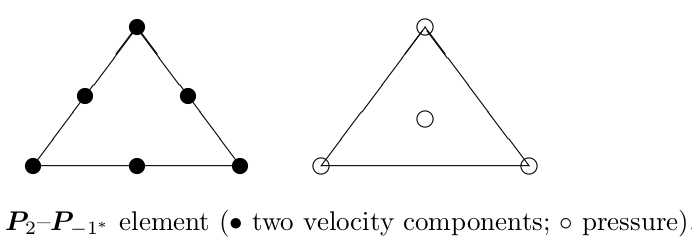
\includegraphics[width=7cm]{images/pair_p2p1p0/elsw}\\
{\captionfont Taken from \textcite{elsw}.}
\end{center}

In Gresho \& Sani table 3.13-1: ``LBB stable yes. Better than P2P1, element mass balance.
more work than P2P1. 2 hydrostatic modes. Second order.'' 

\begin{center}
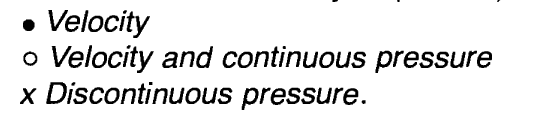
\includegraphics[width=4cm]{images/pair_p2p1p0/grsa2}
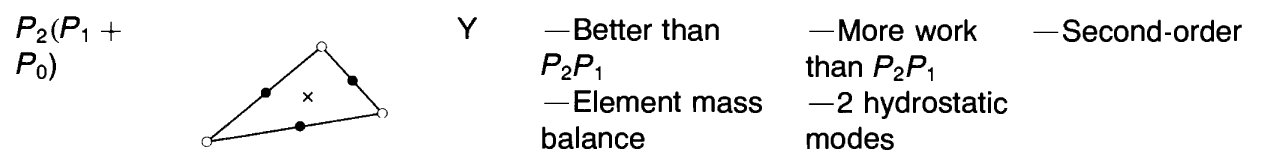
\includegraphics[width=12cm]{images/pair_p2p1p0/grsa1}\\
{\captionfont Taken from \textcite{grsa}. Unfortunately they do not provide a source for 
its origin, for the LBB-stability proof, or any source at all, actually.}
\end{center}

Looking at the figure above, it is clear that the $P_1$ space is to be understood 
as a continuous pressure space, with an additional constant bubble. 

For the continuous $P_1$ space, we have the following reference element
\begin{center}
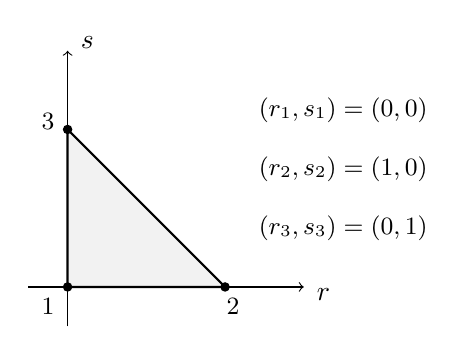
\begin{tikzpicture}
\draw[fill=gray!10,gray!10] (0.5,0.5)--(2.5,0.5)--(0.5,2.5)--cycle;
\draw[thick] (0.5,0.5)--(2.5,0.5)--(0.5,2.5)--cycle;
\draw [->] (0,0.5) -- (3.5,0.5);
\draw [->] (0.5,0) -- (0.5,3.5);
\node[] at (3.75,0.4) {$r$};
\node[] at (0.75,3.6) {$s$};
\draw[black,fill=black] (0.5,0.5)   circle (1.5pt);
\draw[black,fill=black] (2.5,0.5)   circle (1.5pt);
\draw[black,fill=black] (0.5,2.5)   circle (1.5pt);
\node[] at (0.25,0.25) {\small $1$};
\node[] at (2.6,0.25) {\small $2$};
\node[] at (0.25,2.6) {\small $3$};
\node[] at (4,2.75) {\small $(r_1,s_1)=(0,0)$};
\node[] at (4,2) {\small $(r_2,s_2)=(1,0)$};
\node[] at (4,1.25) {\small $(r_3,s_3)=(0,1)$};
\end{tikzpicture}
\end{center}
and the basis functions are simply
\begin{eqnarray}
\bN_1(r,s) &=& 1-r-s \\
\bN_2(r,s) &=& r \\
\bN_3(r,s) &=& s 
\end{eqnarray}
with the interpolation requirement $\bN_i(r_j,s_j)=\delta_{ij}$ fulfilled, as well as $\sum_i \bN_i=1$. 

Now, following the figure by Gresho and Sani, I build the reference element for the $P_1+P_0$ space:
\begin{center}
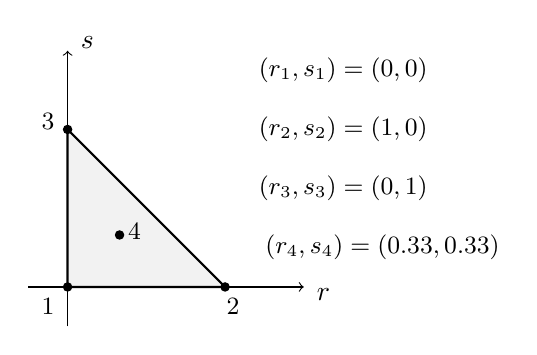
\begin{tikzpicture}
\draw[fill=gray!10,gray!10] (0.5,0.5)--(2.5,0.5)--(0.5,2.5)--cycle;
\draw[thick] (0.5,0.5)--(2.5,0.5)--(0.5,2.5)--cycle;
\draw [->] (0,0.5) -- (3.5,0.5);
\draw [->] (0.5,0) -- (0.5,3.5);
\node[] at (3.75,0.4) {$r$};
\node[] at (0.75,3.6) {$s$};
\draw[black,fill=black] (0.5,0.5)   circle (1.5pt);
\draw[black,fill=black] (2.5,0.5)   circle (1.5pt);
\draw[black,fill=black] (0.5,2.5)   circle (1.5pt);
\draw[black,fill=black] (1.16,1.16) circle (1.5pt);
\node[] at (0.25,0.25) {\small $1$};
\node[] at (2.6,0.25) {\small $2$};
\node[] at (0.25,2.6) {\small $3$};
\node[] at (1.35,1.2) {\small $4$};
\node[] at (4,3.25) {\small $(r_1,s_1)=(0,0)$};
\node[] at (4,2.5)    {\small $(r_2,s_2)=(1,0)$};
\node[] at (4,1.75) {\small $(r_3,s_3)=(0,1)$};
\node[] at (4.5,1) {\small $(r_4,s_4)=(0.33,0.33)$};
\end{tikzpicture}
\end{center}

$P_1+P_0$ means that the pressure inside the element is given by
\[
p^h(r,s) = a \bN_1(r,s)+ b\bN_2(r,s) + c\bN_3(r,s) + d\bN_4(r,s) 
\]
Note that it is then impossible to find $a,b,c,d$ such that the interpolation 
requirement $\bN_i(r_j,s_j)=\delta_{ij}$ is fulfilled.
In other words, the element is not interpolatory, i.e., there is no $\delta_{ij}$ property.% W.B. email

With regards to the 'element mass balance', W.B. states : 
``the mass conservation requires that the function that is constant 1 
on one cell and zero on all other cells is part of the function space. 
That is indeed true -- it's the $\bN_4$ function. Indeed, that's the purpose of 
the enrichment with the $P_0$ part. It is not necessary that {\it all} shape functions are discontinuous.''





\textcite{bocg12} (2012) state: ``[...] the pressure space $Q_h$ is defined as the sum of two finite 
element spaces, namely $P_k+P_0$ ($k \ge d- 1$) [...]for the enhanced Hood–Taylor [...]. 
However, it can be easily observed that the sum is not direct, 
since globally constant functions can be represented exactly by means of piecewise 
$P_0$ or continuous $P_k$ ($k \ge 1$) elements.
Concerning the implementation of the method, we avoid the computation of the basis
functions of such a finite element by testing the discrete problem (2.3) with the basis 
functions of the two subspaces separately. By the above discussion it turns out that the resulting
matrix is rank-deficient, with kernel of dimension 1.''





%------------------------------------------------------------------
\subsubsection{The ${ Q}_2\times (Q_1+Q_0)$ pair} \label{ss:q2q1q0}
It is a rather peculiar element pair (triplet?). The velocity space is the standard $Q_2$ space
but the pressure space is the sum of two spaces, i.e. $Q_1$ {\it and} $Q_0$.
Please see Section~\ref{ss:p2p1p0} on the $P_2\times (P_1+P_0)$ element.

\begin{center}
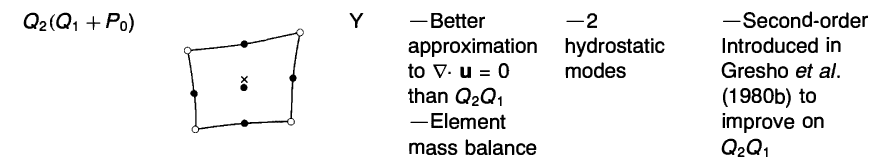
\includegraphics[width=9cm]{images/pair_q2q1q0}\\
{\captionfont Taken from \textcite{grsa}'s book.}
\end{center}

It is implemented in \stone~120.


%------------------------------------------------------------------
\subsubsection{The ${ P}_3\times P_2$ pair} \label{ss:p3p2}
\index{general}{$P_3\times P_2 element$}

${\bm P}_3\times P_2$ mentioned in \cite{sten90}.
The $P_3$ basis functions are presented in Section~\ref{basis:p3} and the $P_2$ basis
functions in Section~\ref{basis:p2}.
See \stone~120


%------------------------------------------------------------------
\subsubsection{The Raviart-Thomas family} \label{ss:raviart_thomas}

- Raviart Thomas 0 RT0 \cite{rath77} ? mentioned/defined/drawn in 4.2.2 of 
Kanschat book. Also exist for quads see 4.2.37 
\textcite{hald03}: ``$P_1^\perp \times P_0$ symbol denotes an element with 
normal velocity nodes in the middle of each edge of the
triangulation [...]. This element, also called low order Raviart–Thomas element 
(Raviart and Thomas, 1977), is based on flux conservation on elements edges and 
the resulting scheme is very close to a finite volume scheme.''

Mentioned in \textcite{john16}, appendix B.3, example B.45: ``the normal component of v 
on each face is a constant. The normal component of functions from RT0 is
continuous across faces of the mesh cells.''

Check \textcite{brfo}


%------------------------------------------------------------------
\subsubsection{The Bernaudi-Raugel pair} \label{ss:bernaudi_raugel}

- from \textcite{cakp15}: The BR-FEM after Bernardi and Raugel \cite{bera85} is a modification of the P2P0 - FEM.
It is sometimes also called reduced $P_2\times P_0$ -FEM \cite{cakp15}

\textcite{bera85} (1985); 

\textcite{cakp15} (2015) state that this element also exists in 3D.

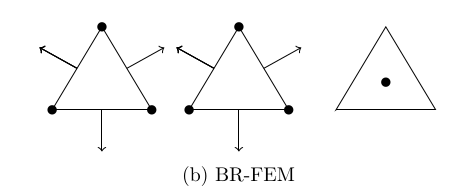
\includegraphics[width=5cm]{images/pair_bernardi_raugel/cakp15}

It is also mentioned in \textcite{bobf13} although it seems it is there called the SMALL element (p474).

In Lederer: "Consider the case d = 2. Above exam-
ple shows, that we only need to control the normal velocity at the edge, i.e. adding the
edge bubble for both components of the velocity seems to be sub optimal (with respect to
computational costs and the expected approximation properties). The idea now is to only
add the normal edge bubble."




%------------------------------------------------------------------
\subsubsection{The Scott-Vogelius pair} \label{ss:scott_vogelius}

\textcite{scvo85} element, see John \cite[p70]{john16}. see \textcite{jolm17} (2017)

- scott-vogelius ? Chen says: ($P^k ,P^{k-1}$) : stable if $k \ge 4$ in $R^2$ and for meshes without
singular-vertex. Exact divergence free. Not easy to code due to the high degree.


%------------------------------------------------------------------
\subsubsection{The BDM (Brezzi-Douglas-Marini) pair} \label{ss:bdm}
\index{general}{BDM element}

- BDM (Brezzi-Douglas-Marini)mentioned in Kanschat book 4.2.14. 
Also exist for quads see 4.2.39

Mentioned in \textcite{chen93a} (1993).

Check \textcite{brfo}


%------------------------------------------------------------------
\subsubsection{The DSSY pair} \label{ss:pair_dssy2D}
\index{general}{Nonconforming element}
\index{general}{DSSY element}
This element is often referred to as the 'DSSY' element because of the 
four authors of the original paper: Douglas, Santos, sheen and Ye (1999) \cite{doss99}.

The non-conforming finite element space $Q_l$ is defined based on the 
reference square element on $[-1,1]^2$ :
\[
Q_l = \text{Span} \left\{ 1, r, s, \theta_l(r)-\theta_l(s)  \right\}
\qquad l=1,\; \text{or} \; 2
\]
with
\begin{eqnarray}
\theta_1(r)  &=& r^2-\frac53r^4  \nn\\
\theta_1'(r) &=& 2r-\frac{20}{3}r^3  \nn\\
\theta_2(r)  &=& r^2-\frac{25}{6} r^4 + \frac72 r^6 \\ 
\theta_2'(r) &=& 2r-\frac{50}{3} r^3 + 21 r^5
\end{eqnarray}
The dimension of $Q_l$ is four and the $\theta_l$ functions look like:
\begin{center}
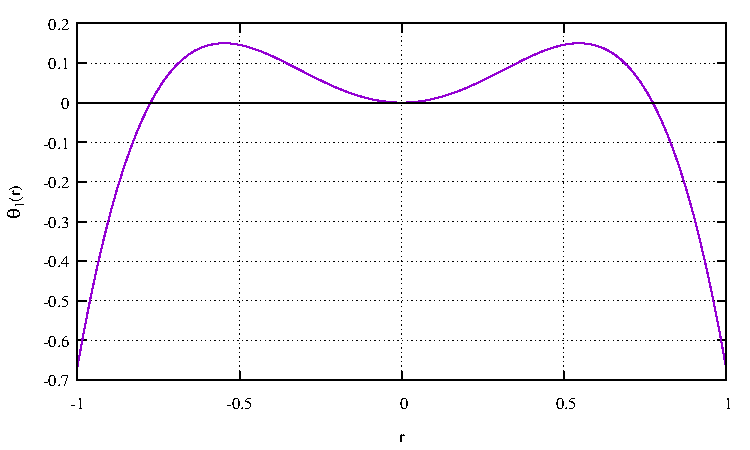
\includegraphics[width=7cm]{images/dssy/theta1}
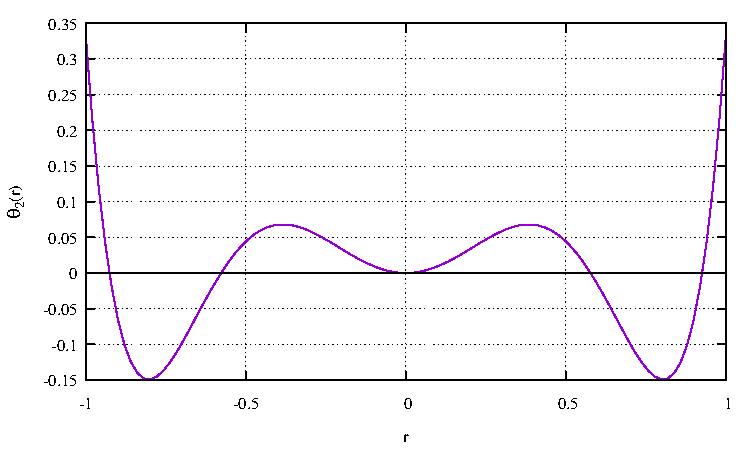
\includegraphics[width=7cm]{images/dssy/theta2}
\end{center}
We have:
\begin{itemize}
\item $\theta_1(r=-1)=\theta_1(r=+1)=-\frac23$, $\theta_1(r=0)=0$ 
\item $\theta_2(r=-1)=\theta_2(r=+1)=\frac13$, $\theta_2(r=0)=0$ 
\end{itemize}
The nodes are situated at the mid-edges of the quadrilateral:

\begin{flushright} {\tiny {\color{gray} (tikz\_dssy2D.tex)}} \end{flushright}
%~~~~~~~~~~~~~~~~~~~~~~~~~~~~~~~~~~~~~~~~~~~~~~~~~~~~~~~~~~~~~~~~~~~~~~~~~~~~~~~~~~~~~~~~~~~~~~~~~~

\begin{center}
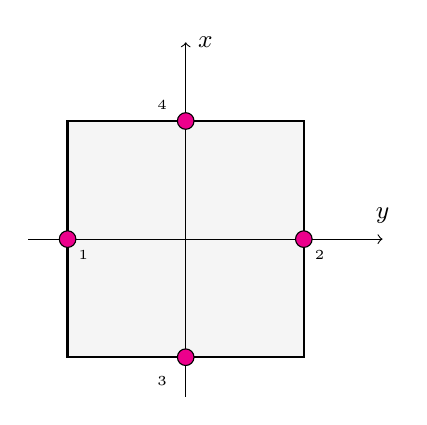
\begin{tikzpicture}
%\draw[step=1cm,gray,very thin] (0,0) grid (8,8); %background grid

\draw[thick,fill=gray!8] (1,1) -- (4,1) -- (4,4) -- (1,4) -- cycle;

\node[] at (1.2,2.3) {\tiny 1};
\node[] at (4.2,2.3) {\tiny 2};
\node[] at (2.2,.7) {\tiny 3};
\node[] at (2.2,4.2) {\tiny 4};

\draw[->] (0.5,2.5)--(5,2.5);
\draw[->] (2.5,0.5)--(2.5,5);

\draw[black,fill=magenta] (1,2.5)   circle (3pt);
\draw[black,fill=magenta] (4,2.5)   circle (3pt);
\draw[black,fill=magenta] (2.5,1)   circle (3pt);
\draw[black,fill=magenta] (2.5,4)   circle (3pt);

\node[] at (5,2.8) {\small $y$};
\node[] at (2.75,5) {\small $x$};
\end{tikzpicture}
\end{center}




The basis function corresponding to the node (1, 0) is given by
\begin{mdframed}[backgroundcolor=blue!5]
\begin{eqnarray}
\bN_1(r,s)^{(l)} &=& \frac{1}{4} - \frac{1}{2} r + \frac{\theta_l(r)-\theta_l(s)}{4 \theta_l(1)}  \nn\\
\bN_2(r,s)^{(l)} &=& \frac{1}{4} + \frac{1}{2} r + \frac{\theta_l(r)-\theta_l(s)}{4 \theta_l(1)}  \nn\\
\bN_3(r,s)^{(l)} &=& \frac{1}{4} - \frac{1}{2} s - \frac{\theta_l(r)-\theta_l(s)}{4 \theta_l(1)}  \nn\\
\bN_4(r,s)^{(l)} &=& \frac{1}{4} + \frac{1}{2} s - \frac{\theta_l(r)-\theta_l(s)}{4 \theta_l(1)}  
\end{eqnarray}
\end{mdframed}
We can easily verify that $\sum\limits_i \bN_i(r,s,t)=1$ and that $\bN_i(\vec{r}_j)=\delta_{ij}$:
\begin{eqnarray}
\bN_1^{(l)}(r_1,s_1) 
&=& \frac{1}{4} -\frac{1}{2} (-1) + \frac{\theta_l(-1)-\theta_l(0)}{4 \theta_l(1)}  
= \frac{1}{4} +\frac{1}{2}  + \frac{\theta_l(-1)}{4 \theta_l(1)}  
= \frac{1}{4} +\frac{1}{2}  + \frac{1}{4}   = 1 \nn\\
\bN_1^{(l)}(r_2,s_2)
&=& \frac{1}{4} -\frac{1}{2} (+1) + \frac{\theta_l(+1)-\theta_l(0)}{4 \theta_l(1)}  
= \frac{1}{4} -\frac{1}{2} + \frac{\theta_l(+1)}{4 \theta_l(1)}  
= \frac{1}{4} -\frac{1}{2} + \frac{1}{4}   = 0 \nn\\
\bN_1^{(l)}(r_3,s_3)
&=& \frac{1}{4} -\frac{1}{2} (0) + \frac{\theta_l(0)-\theta_l(-1)}{4 \theta_l(1)}  
= \frac14 -\frac14  = 0 \nn\\
\bN_1^{(l)}(r_4,s_4)
&=& \frac{1}{4} -\frac{1}{2} (0) + \frac{\theta_l(0)-\theta_l(+1)}{4 \theta_l(1)}  
= \frac14 -\frac14  = 0 \nn\\
\bN_2^{(l)}(r_1,s_1) 
&=& \frac{1}{4} + \frac{1}{2} (-1) + \frac{\theta_l(-1)-\theta_l(0)}{4 \theta_l(1)}  
= \frac14 -\frac12 + \frac14 = 0 \nn\\
\bN_2^{(l)}(r_2,s_2)
&=& \frac{1}{4} + \frac{1}{2} (+1) + \frac{\theta_l(+1)-\theta_l(0)}{4 \theta_l(1)}  
= \frac14 + \frac12 + \frac14 =1 \nn\\
\bN_2^{(l)}(r_3,s_3)
&=& \frac{1}{4} + \frac{1}{2} (0) + \frac{\theta_l(0)-\theta_l(-1)}{4 \theta_l(1)}  
= \frac14 - \frac14 = 0 \nn\\
\bN_2^{(l)}(r_4,s_4)
&=& \frac{1}{4} + \frac{1}{2} (0) + \frac{\theta_l(0)-\theta_l(+1)}{4 \theta_l(1)}  
= \frac14 - \frac14 = 0 \nn\\
\bN_3^{(l)}(r_1,s_1)
&=& \frac{1}{4} - \frac{1}{2} (0) - \frac{\theta_l(-1)-\theta_l(0)}{4 \theta_l(1)} 
= \frac14 -\frac14 = 0\nn\\
\bN_3^{(l)}(r_2,s_2)
&=& \frac{1}{4} - \frac{1}{2} (0) - \frac{\theta_l(+1)-\theta_l(0)}{4 \theta_l(1)} 
= \frac14 -\frac14 = 0\nn\\
\bN_3^{(l)}(r_3,s_3)
&=& \frac{1}{4} - \frac{1}{2} (-1) - \frac{\theta_l(0)-\theta_l(-1)}{4 \theta_l(1)} 
= \frac14 +\frac12 + \frac14 = 1\nn\\
\bN_3^{(l)}(r_4,s_4)
&=& \frac{1}{4} - \frac{1}{2} (+1) - \frac{\theta_l(0)-\theta_l(+1)}{4 \theta_l(1)} 
= \frac14 -\frac12 + \frac14 = 0\nn\\
\bN_4^{(l)}(r_1,s_1)
&=& \frac{1}{4} + \frac{1}{2} (0) - \frac{\theta_l(-1)-\theta_l(0)}{4 \theta_l(1)}  
= \frac14 -\frac14 =0\nn\\
\bN_4^{(l)}(r_2,s_2)
&=& \frac{1}{4} + \frac{1}{2} (0) - \frac{\theta_l(+1)-\theta_l(0)}{4 \theta_l(1)}  
= \frac14 -\frac14 =0\nn\\
\bN_4^{(l)}(r_3,s_3)
&=& \frac{1}{4} + \frac{1}{2} (-1) - \frac{\theta_l(0)-\theta_l(-1)}{4 \theta_l(1)}  
= \frac14 -\frac12 +\frac14 = 0 \nn\\
\bN_4^{(l)}(r_4,s_4)
&=& \frac{1}{4} + \frac{1}{2} (1) - \frac{\theta_l(0)-\theta_l(1)}{4 \theta_l(1)}  
= \frac14 +\frac12 +\frac14 = 1 \nn
\end{eqnarray}

The basis functions can also be explicitly written for $\theta_1$ as in Cai \etal \cite{cady99}:
\begin{eqnarray}
\bN_1(r,s)^{(l)} 
&=& \frac{1}{4} - \frac{1}{2} r - \frac38 \left[\left( r^2-\frac53r^4 \right) - \left(s^2-\frac53s^4 \right) \right] \nn\\
\bN_2(r,s)^{(l)} 
&=& \frac{1}{4} + \frac{1}{2} r - \frac38 \left[\left( r^2-\frac53r^4 \right) - \left(s^2-\frac53s^4 \right) \right] \nn\\
\bN_3(r,s)^{(l)} 
&=& \frac{1}{4} - \frac{1}{2} s + \frac38 \left[\left( r^2-\frac53r^4 \right) - \left(s^2-\frac53s^4 \right) \right] \nn\\
\bN_4(r,s)^{(l)} 
&=& \frac{1}{4} + \frac{1}{2} s + \frac38 \left[\left( r^2-\frac53r^4 \right) - \left(s^2-\frac53s^4 \right) \right] 
\end{eqnarray}

The derivatives of the basis functions are as follows:
\begin{eqnarray}
\partial_r \bN_1(r,s)^{(l)} &=&  - \frac{1}{2}  + \frac{\theta_l'(r)}{4 \theta_l(1)}  \nn\\
\partial_r \bN_2(r,s)^{(l)} &=&  + \frac{1}{2}  + \frac{\theta_l'(r)}{4 \theta_l(1)}  \nn\\
\partial_r \bN_3(r,s)^{(l)} &=&  - \frac{\theta_l'(r)}{4 \theta_l(1)}  \nn\\
\partial_r \bN_4(r,s)^{(l)} &=&  - \frac{\theta_l'(r)}{4 \theta_l(1)}  
\end{eqnarray}

\begin{eqnarray}
\partial_s \bN_1(r,s)^{(l)} &=&   -\frac{\theta_l'(s)}{4 \theta_l(1)}  \nn\\
\partial_s \bN_2(r,s)^{(l)} &=&   -\frac{\theta_l'(s)}{4 \theta_l(1)}  \nn\\
\partial_s \bN_3(r,s)^{(l)} &=&   - \frac{1}{2} + \frac{\theta_l'(s)}{4 \theta_l(1)}  \nn\\
\partial_s \bN_4(r,s)^{(l)} &=&   + \frac{1}{2} + \frac{\theta_l'(s)}{4 \theta_l(1)}  
\end{eqnarray}





\Literature: 
Park \& Sheen (2003) \cite{pash03},
Jeon \etal (2013) \cite{jens13},
Park, Sheen \& Shin (2013) \cite{pass13},
Bangerth \etal (2017) \cite{baks17},
Sheen (2020) \cite{shee20}


%------------------------------------------------------------------
\subsubsection{The Han pair} \label{ss:han}
\index{general}{Han element}
\index{general}{Nonconforming element}


It is based on \textcite{han84} (also mentioned in Sheen (2020) \cite{shee20}).
The nodes are at the same location as for the RT element above, but 
there is an additional bubble function in the middle:
\begin{verbatim}
+====3====+
|         |
4    5    2
|         |
+====1====+
\end{verbatim}
Inside the reference element we assume that a field $f$
can be represented by 
\begin{eqnarray}
f^h(r,s) 
&=& a+ br +cs +d \phi(r) +e \phi(s) \nn\\
&=& a+ br +cs +d \frac{5r^4-3r^2}{2}+e \frac{5s^4-3s^2}{2} \nn
\end{eqnarray}
We then must have 
\begin{eqnarray}
f_1 = f^h(r=1,s=0) &=& a+ b +d \nn\\
f_2 = f^h(r=0,s=1) &=& a+ c +e \nn\\
f_3 = f^h(r=-1,s=0) &=& a- b +d \nn\\
f_4 = f^h(r=0,s=-1) &=& a -c +e \nn\\
f_5 = f^h(r=0,s=0) &=& a  \nn
\end{eqnarray}
and we easily get 
\[
a = f_5 
\qquad
f_1-f_3 = 2b
\qquad 
f_2-f_4 = 2c
\]
followed by
\[
d=f_1-a-b = f_1 - f_5 - \frac{1}{2}(f_1-f_3) = \frac{f_1-2f_5+f_3}{2}
\]
and 
\[
e = f_2-a-c = f_2 - f_5 -  \frac{1}{2}(f_2-f_4) = \frac{f_2 -2f_5+f_4 }{2}
\]
Finally:
\[
f(r,s) = 
f_5 +
\frac{1}{2}(f_1-f_3) r+
\frac{1}{2}(f_2-f_4) s+
\frac{f_1-2f_5+f_3}{2} \phi(r)+
\frac{f_2 -2f_5+f_4 }{2} \phi(s)
\]
i.e.
\[
f(r,s) = 
\left(\frac{r + \phi(r)}{2} \right)f_1 +
\left(\frac{s+\phi(s)}{2} \right)f_2 +
\left(-\frac{r-\phi(r)}{2} \right)f_3 +
\left(-\frac{s - \phi(s)}{2} \right)f_4 +
\left(1-\phi(r)-\phi(s) \right)f_5 
\]
which has us define 
\begin{eqnarray}
\bN_1(r,s) &=& \frac{r + \phi(r)}{2} \nn\\
\bN_2(r,s) &=& \frac{s+\phi(s)}{2} \nn\\
\bN_3(r,s) &=& -\frac{r-\phi(r)}{2} \nn\\
\bN_4(r,s) &=& -\frac{s - \phi(s)}{2}\nn\\
\bN_5(r,s) &=& 1-\phi(r)-\phi(s)\nn
\end{eqnarray}
We have of course the following properties $\sum_{i=1}^5 \bN_i(r,s) = 1$ and 
$\bN_i(r_j,s_j) = \delta_{ij}  \qquad i,j \in 1,5$. 
The partial derivatives of the basis functions are as follows
\begin{eqnarray}
\partial_r \bN_1(r,s) &=& \frac{1 + \phi'(r)}{2} \nn\\
\partial_r \bN_2(r,s) &=& 0 \nn\\
\partial_r \bN_3(r,s) &=& -\frac{1-\phi'(r)}{2} \nn\\
\partial_r \bN_4(r,s) &=& 0 \nn\\
\partial_r \bN_5(r,s) &=& -\phi'(r) \nn\\
\partial_s \bN_1(r,s) &=& 0 \nn\\
\partial_s \bN_2(r,s) &=& \frac{1 + \phi'(s)}{2} \nn\\
\partial_s \bN_3(r,s) &=&  0 \nn\\
\partial_s \bN_4(r,s) &=& -\frac{1-\phi'(s)}{2} \nn\\
\partial_s \bN_5(r,s) &=& -\phi'(s) \nn
\end{eqnarray}
This element is implemented in the {\tt stone\_han.py} file in \stone~77 and also in \stone~120. 








%------------------------------------------------------------------
\subsubsection{The Divergence-free nonconforming $P_1^{NC}\times P_0$ pair} \label{ss:p1ncp0}

INSERT FIGURE OF DOFS

It belongs to the Crouzeix-Raviart family. 
The midside nodes are used as degrees of freedom for the velocities.
It is mentioned in Section~6.3 of \textcite{bobf08} (2008): ``[...]
It is exactly divergence free. Another important feature of this
element is that it can be seen as a "mass conservation" scheme. The present element
has been generalized to second order in \textcite{foso83} (1983).
It must also be said that coerciveness may be a problem for the $P_1^{NC} \times P_0$ 
element, as it does not satisfy the discrete version of Korn’s inequality. 
This issue has been deeply investigated and clearly illustrated in \textcite{arno93} (1993).''

At page 170 of \cite{braess} it is stated that ``an analogous quadrilateral element was 
developed and studied by \textcite{ratu92} (1992)''.

\textcite{bobf13}: ``We consider the classical (almost) stable nonconforming triangular 
element introduced in \textcite{crra73}, in which mid-side nodes are used as degrees of 
freedom for the velocities. This generates
a piecewise linear nonconforming approximation; pressures are taken constant on
each element. It is also possible to build a three-dimensional
version of this element, using mid-face nodes as degrees of freedom.''
Also: ``It must also be recalled that coercivity is a problem for the $P_1^{NC}\times P_0$ 
element. The trouble is that the bilinear form (8.2.1) is not coercive on the 
nonconforming space $V_h$ and we do not have the discrete version of Korn's inequality.''

It is also mentioned in \textcite{john16}, appendix B.3, example B.43, in 2D and 3D, 
in \textcite{brfo} (example 8.1), and studied extensively in \textcite{john98} (1998). 

\begin{center}
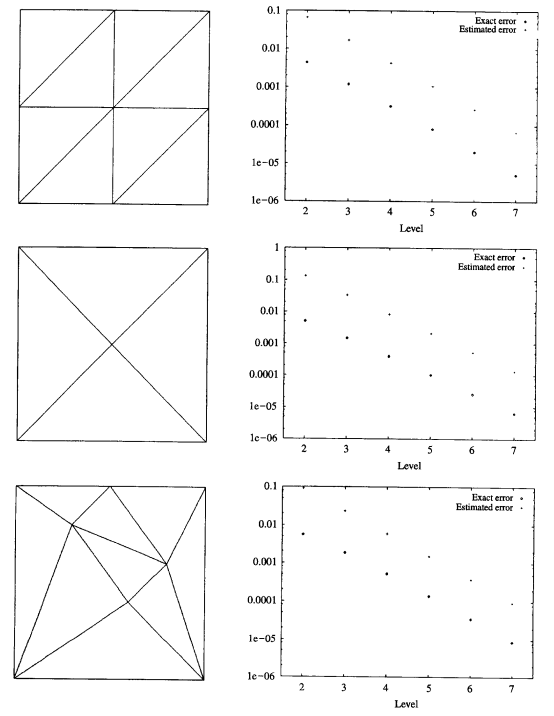
\includegraphics[width=8cm]{images/pair_p1ncp0/john98}\\
{\captionfont Taken from \textcite{john98}.}
\end{center}



%------------------------------------------------------------------
\subsubsection{The Chen nonconforming ${ Q}_1\times Q_0$ pair (?)} \label{ss:chenq0}
\begin{flushright} {\tiny {\color{gray} pair\_chen.tex}} \end{flushright}
%~~~~~~~~~~~~~~~~~~~~~~~~~~~~~~~~~~~~~~~~~~~~~~~~~~~~~~~~~~~~~~~~~~~~~~~~~~~~~~~~~~~~~~~~~~~~~~~~~~

What follows is tentative!

This space is proposed in \textcite{chen93} (1993), albeit not in the 
context of the Stokes equations.

It is based on the mid-point variant of the RT basis functions, 
\begin{eqnarray}
\bN_1(r,s) &=& \frac{1}{4} (1-2s-(r^2-s^2)) \nonumber\\
\bN_2(r,s) &=& \frac{1}{4} (1+2r+(r^2-s^2)) \nonumber\\
\bN_3(r,s) &=& \frac{1}{4} (1+2s-(r^2-s^2)) \nonumber\\
\bN_4(r,s) &=& \frac{1}{4} (1-2r+(r^2-s^2)) \nonumber
\end{eqnarray}
to which a $P_2$ bubble is added
\[
\phi(r,s) = 1-\frac34(r^2+s^2)
\]
Note thath this function is zero at locations $\pm 1/\sqrt{3}$ 
on all four edges and exactly 1 in the middle. 

A field $f$ is represented inside the element by 
\[
f^h(r,s)=a \bN_1(r,s)
+b \bN_2(r,s)
+c \bN_3(r,s)
+d \bN_4(r,s)
+e \phi(r,s)
\]
We immediately see that this space is not interpolatory, i.e. the basis function $\phi(r,s)$ cannot be 1 in the middle and 0 at the other four nodes. 

\textcite{chen} also extends this to 3D in the paper. 

This space is used for velocity and a $Q_0$ space is used for 
pressure in \stone~120 (only because the basis functions above are
based on the Rannacher-Turek ones).


%----------------------------
\subsubsection{Other FE element pairs}

\begin{itemize}

\item ${\bm Q}_2\times Q_2$: This element is never used, probably because 
a) it is unstable, b) it is very costly. 
There is one reference to it in \cite{hufb86}.

\item ${\bm Q}_1\times P_{-1}$ Bilinear velocities,  piecewise linear discontinuous polynomial pressure.

\item See Fortin \cite{fort81} for various stable low order elements other than the enriched 
${\bm Q}_1^+ \times P_0$

\item ${\bm Q}_1\times Q_1$ + nonconforming null edge average \cite{fros07}

\item check \textcite{dhhu86} (1986) many flavours of triangles and quads.

\item Bercovier-Pironneau element pair, or $P_1isoP_2$.See \textcite{bocg12} (2012).

\end{itemize}

%.........................................................................
\subsubsection{A note about incompressibility and standard mixed methods}

What follows is nicely explained and demonstrated in John \etal \cite{jolm17}. In their 
example 1.1 they look at the velocity error of benchmark VJ2 (see Section~\ref{mms9}) 
which analytical solution is a zero velocity field. They show that for the MINI, 
Taylor-Hood and Crouzeix-Raviart triangular elements the velocity error grows 
with the magnitude of the rhs. They also make this statement:
\say{
there are important applications, e.g., natural
convection problems, where the pressure is larger than the velocity by orders
of magnitude. In such situations, one cannot expect to compute accurate
velocity fields with classical mixed methods, at least for low order methods.
}


